% !TeX root = ../../Book5.tex
% 纲要标题：## 第1章　仿射、射影与有理几何的模型
% 纲要位置：几何学计划纲要.md，第 5028 行。
% 正文状态：初稿；尚未正式审核。

% 纲要内容开始
% 
% > 本章目标与证明范围：把经典几何入口合成有实质内容的一章：方程—函数—映射—消去—射影紧化。初始取代数闭域，进入概形后再系统改变基域；不把投影像等同于消去得到的闭包。
% 
% 纲要内容结束

\chapter{仿射、射影与有理几何的模型}
\label{g5:ch:01}
\BookChapterNumber{g5:ch:01}

\begin{chapterabstract}
	多项式方程既给出点集，也给出点上及点附近可以使用的函数。本章先证明多项式环的有限性与零点定理，建立仿射代数集和约化坐标环的反变对应，再以正则函数、函数域和稠密开集比较几何模型。射影坐标把乘积、子空间及曲线参数实现为齐次方程；多元除法、Gröbner 基和消去计算则从方程及参数中提取映射像的闭包。最后用结点、尖点、无穷远分支及重合纤维，说明点集、函数域与局部代数各自保留的信息。
\end{chapterabstract}

\begin{learninggoals}
	\begin{itemize}
		\item 证明多项式环的理想有限生成，使用弱、强零点定理把零点条件转换成理想条件，并找出不可约分量。
		\item 从局部分式判断函数与映射的正则性，以坐标环同态和函数域嵌入分别描述正则映射与支配有理映射。
		\item 写出射影仿射图、Segre 与 Veronese 嵌入及 Plücker 关系，并由像坐标恢复原来的几何对象。
		\item 完成多元除法和 Buchberger 算法，计算消去理想、饱和与有限商代数，区分实际投影像及其闭包。
		\item 在具体曲线与纤维中辨认分支、延拓障碍和幂零信息，说明局部环及保留方程的纤维为何必要。
	\end{itemize}
\end{learninggoals}

方程 \(xy=1\) 的每个非零横坐标都对应唯一纵坐标 \(y=1/x\)，但横坐标 \(0\) 没有原像。若只寻找所有横坐标共同满足的多项式方程，结果却是零理想：一个在所有非零元素处消失的一元多项式必为零。因此，方程可以准确描述这条曲线，却不能只靠横坐标上的方程描述其投影像；从方程消去变量时，必须知道所得对象与原来的点集有什么关系。

\ProseParagraphBreak

另一个变化发生在 \(t\mapsto(t^2,t^3)\)。这个参数把直线上的点一一映到 \(y^2=x^3\)，而逆参数 \(y/x\) 在原点附近不能用不消失的分母表示。两空间有相同的有理函数域，却有不同的局部函数。再看 \(x=0\) 和 \(x^2=0\)：二者零点相同，方程取商得到的环却不同。由方程到函数、再由函数理解映射，能够同时处理这些现象。

\ProseParagraphBreak

本章所需基础是域、理想、商环、域扩张以及有限维线性代数，并使用一元多项式带余除法、因式分解和行列式。开集、闭集、连续性、不可约性会在所研究的空间中说明。初始基域 \(k\) 取代数闭域；纯多项式算法及若干代数引理在陈述中给出较一般的基域条件，结点和纤维计算则逐处注明特征。仿射代数集允许可约，非空不可约者称为仿射簇。局部化、模和概形的一般理论随后建立，本章先通过可直接计算的模型引出它们。

\ProseParagraphBreak

仿射与射影簇、正则映射和有理映射可对照\cite[第I章第1--4节]{Hartshorne1977}；典型射影嵌入还可对照\cite[第1章第4节]{Shafarevich2013Basic1}。计算方法的阅读位置随\secref{g5:sec:0104}各项构造列出。本章完整证明所用的有限性、零点对应、映射对应及消去结论，曲线与有限商代数的算例将贯穿这些证明。

% !TeX root = ../../Book5.tex
% 纲要标题：### 1.1 方程与坐标环
% 纲要位置：几何学计划纲要.md，第 4738 行。
% 正文状态：未撰写；本文件目前是框架。

% 纲要内容开始
% 
% * Zariski 拓扑、理想和根式
% * Hilbert 基定理的有限性证明
% * 弱零点定理与 Zariski 引理
% * 强零点定理的 Rabinowitsch 论证
% * 不可约分支及反变对应
% 
% 纲要内容结束

\section{方程与坐标环}
\label{g5:sec:0101}

待撰写

\subsection{Zariski 拓扑、理想和根式}
\label{g5:subsec:0101:01}
待撰写

\subsection{Hilbert 基定理的有限性证明}
\label{g5:subsec:0101:02}
待撰写

\subsection{弱零点定理与 Zariski 引理}
\label{g5:subsec:0101:03}
待撰写

\subsection{强零点定理的 Rabinowitsch 论证}
\label{g5:subsec:0101:04}
待撰写

\subsection{不可约分支及反变对应}
\label{g5:subsec:0101:05}
待撰写
% 纲要条目排为编号小节标题，并进入目录与书签；说明段仍保留于纲要注释中。

% !TeX root = ../../Book5.tex
% 纲要标题：### 1.2 正则与有理映射
% 纲要位置：几何学计划纲要.md，第 5040 行。
% 正文状态：未撰写；本文件目前是框架。

% 纲要内容开始
% 
% * 正则函数和局部表达
% * 函数域及支配有理映射
% * 双有理等价和稠密开集
% * 图像、未定义点及延拓障碍
% 
% 纲要内容结束

\section{正则与有理映射}
\label{g5:sec:0102}

待撰写

\subsection{正则函数和局部表达}
\label{g5:subsec:0102:01}
待撰写

\subsection{函数域及支配有理映射}
\label{g5:subsec:0102:02}
待撰写

\subsection{双有理等价和稠密开集}
\label{g5:subsec:0102:03}
待撰写

\subsection{图像、未定义点及延拓障碍}
\label{g5:subsec:0102:04}
待撰写
% 纲要条目排为编号小节标题，并进入目录与书签；说明段仍保留于纲要注释中。

% !TeX root = ../../Book5.tex
% 纲要标题：### 1.3 射影空间与典型嵌入
% 纲要位置：几何学计划纲要.md，第 5047 行。
% 正文状态：初稿；尚未正式审核。

% 纲要内容开始
% 
% * 齐次方程和仿射图
% * Segre、Veronese 及其方程
% * Grassmann 与 Plücker 关系
% * 射影曲线及有理参数
% 
% 纲要内容结束

\section{射影空间与典型嵌入}
\label{g5:sec:0103}

在仿射平面中，双曲线 \(xy=1\) 的投影漏掉原点；一条直线的斜率也不能记录竖直方向。把坐标改成比例，可以把这些遗漏的方向作为点保存。新的问题随即出现：比例坐标满足什么方程，如何与仿射计算衔接，又怎样用一个点记录一对子空间或一个高次表达式？本节仍取代数闭域 \(k\)，从齐次方程建立射影模型，再把乘积、子空间和曲线参数写成可恢复的坐标。

\subsection{齐次方程和仿射图}
\label{g5:subsec:0103:01}

\begin{definition}
\label{g5:def:projective-space}
	设 \(k\) 为代数闭域，\(n\geq0\)。非零向量 \(k^{n+1}\setminus\{0\}\) 在关系 \(x\sim\lambda x\)（\(\lambda\in k^\times\)）下的商集称为 \(k\) 上的 \(n\) 维\term[sheyingkongjian]{射影空间}[projective space]，记为 \(\mathbb P^n_k\)。点写作 \([x_0:\cdots:x_n]\)，其中的 \(x_i\) 称为\term[qicizuobiao]{齐次坐标}[homogeneous coordinates]。
	\symidx{\(\mathbb P^n_k\)：域 \(k\) 上的射影空间}
\end{definition}

一个射影点等价地是一条通过原点的向量直线。这里共同倍数可以改变，单独一个坐标的值没有不依赖代表的意义。若 \(F\in k[x_0,\ldots,x_n]\) 是 \(d\) 次齐次多项式，则 \(F(\lambda x)=\lambda^dF(x)\)，所以条件 \(F(x)=0\) 却与代表无关。对一族齐次多项式 \(\mathcal F\)，定义
\[
	V_+(\mathcal F)=\{[x]\in\mathbb P^n_k:F(x)=0\text{ 对所有 }F\in\mathcal F\}.
\]
这些集合满足闭集公理：任意交对应合并方程，两个零点集的并对应两族方程的所有乘积；空集由 \(x_0=\cdots=x_n=0\) 给出，全集由零多项式给出。由此得到射影空间的 Zariski 拓扑。其闭集称为\term[sheyingdaishuji]{射影代数集}[projective algebraic set]；非空不可约的射影代数集称为\term[sheyingcu]{射影簇}[projective variety]。

把多项式按总次数分解成齐次部分，就有 \(k[x_0,\ldots,x_n]=\bigoplus_{d\geq0}S_d\)。由齐次多项式生成的理想称为\term[qicilixiang]{齐次理想}[homogeneous ideal]。每个元素的齐次部分仍在这个理想中，因为把生成式中的系数也逐次分解即可。射影方程因此可记为 \(V_+(J)\)，其中 \(J\) 是齐次理想。Hilbert 基定理保证方程可取有限个齐次生成元：先取有限生成元，再取它们的全部齐次部分。

\begin{proposition}
\label{g5:prop:projective-affine-charts}
	设 \(k\) 为代数闭域，\(n\geq1\)。开集 \(U_i=\{x_i\ne0\}\subseteq\mathbb P^n_k\) 覆盖 \(\mathbb P^n_k\)，而映射
	\[
		\phi_i:U_i\longrightarrow\mathbb A^n_k,\qquad
		[x_0:\cdots:x_n]\longmapsto(x_0/x_i,\ldots,\widehat{x_i/x_i},\ldots,x_n/x_i)
	\]
	是同胚。在两张图的交上，坐标变换及其逆都由分母不为零的多项式商给出。
\end{proposition}
\begin{proof}
	至少有一个坐标非零，所以这些开集覆盖全部点。\(\phi_i\) 的逆在第 \(i\) 个位置插入 \(1\)，故它是双射。齐次方程 \(F(x)=0\) 在 \(U_i\) 中成为令 \(x_i=1\) 得到的多项式方程。反过来，仿射坐标中的多项式 \(f\) 若次数为 \(d\)，则
	\[
		F(x)=x_i^d f(x_0/x_i,\ldots,\widehat{x_i/x_i},\ldots,x_n/x_i)
	\]
	是齐次多项式，且其在 \(U_i\) 上的零点恰对应 \(V(f)\)。这证明双向连续性。在 \(U_i\cap U_j\) 上写 \(u_\ell=x_\ell/x_i\)，补记 \(u_i=1\)，则第 \(j\) 张图中的坐标为 \(u_\ell/u_j\)，而 \(u_j\ne0\)。交换 \(i,j\) 即得逆变换。
\end{proof}

\(U_i\) 称为一张\term[fangshetu]{仿射图}[affine chart]。这使\secref{g5:sec:0102}的正则函数定义可以用于射影代数集：函数在每张仿射图中局部为多项式商，且分母在所讨论点不为零。图间变换正则，因而此定义不依赖图的选择。射影簇的开子集称为\term[zhunsheyingcu]{准射影簇}[quasi-projective variety]；允许可约时，同样讨论射影代数集的开子集及其正则函数。映射在源、靶的仿射图中为正则映射时，称为正则映射；有正则逆的双射称为同构。

例如，\(\mathbb P^1_k=\mathbb A^1_k\cup\{[0:1]\}\)：在 \(x_0\ne0\) 的图中用 \(t=x_1/x_0\)，另一图用 \(s=x_0/x_1\)，交上的关系是 \(s=1/t\)。每张 \(U_i\) 都在 \(\mathbb P^n_k\) 中稠密。事实上，若一个齐次多项式在 \(U_i\) 上为零，其去齐次化在 \(k^n\) 上恒为零；无限域上的多项式恒等原理表明该多项式为零，再齐次化就得到原式为零。仿射空间不可约，因此其稠密闭包 \(\mathbb P^n_k\) 也不可约。

若 \(F_0,\ldots,F_m\) 是同次齐次多项式，则
\[
	[x]\longmapsto[F_0(x):\cdots:F_m(x)]
\]
在这些多项式不同时为零的开集上定义正则映射：在 \(F_j\ne0\) 的靶图中，坐标恰是 \(F_i/F_j\)。共同零点处的公式不能直接赋值；能否换用别的局部表达来延拓，要另行检查。本节末的曲线会给出一个可以延拓的例子。

上述齐次方程与仿射图的构造可对照\cite[第I章，第2节，命题2.1--2.2]{Hartshorne1977}。

\subsection{Segre、Veronese 及其方程}
\label{g5:subsec:0103:02}

考虑一对射影点 \([x]\in\mathbb P^m_k\)、\([y]\in\mathbb P^n_k\)。把两组坐标直接并排，不能消去它们各自独立的缩放；取乘积 \(x_i y_j\) 则使两次缩放合成一个共同倍数。乘积 \(\mathbb P^m_k\times\mathbb P^n_k\) 用图 \(U_a\times U_b\cong\mathbb A^{m+n}_k\) 赋予代数几何结构，正则性按这些图检验。两组坐标分别换图，所以转换公式仍为分母非零的多项式商。这里的 Zariski 拓扑由仿射图中的多项式方程确定。

\begin{proposition}
\label{g5:prop:segre-embedding}
	设 \(k\) 为代数闭域，\(m,n\geq0\)。\term[Segreqianru]{Segre 嵌入}[Segre embedding]
	\[
		\sigma:\mathbb P^m_k\times\mathbb P^n_k\longrightarrow\mathbb P^{(m+1)(n+1)-1}_k,
		\qquad([x],[y])\longmapsto[x_i y_j]_{i,j}
	\]
	将其定义域同构到由全部方程
	\[
		z_{ij}z_{ab}-z_{ib}z_{aj}=0
		\qquad(0\leq i,a\leq m,\ 0\leq j,b\leq n)
	\]
	定义的射影代数集。
\end{proposition}

这里嵌入指与一个闭代数子集的同构，因而同时要求像的闭性与逆映射的正则性。Segre 的乘积坐标把这两项要求化为秩一矩阵的恢复。\footnote{Corrado Segre（1863--1924），意大利数学家，研究高维射影几何与代数曲面。}

\begin{proof}
	分别缩放 \(x,y\) 只会共同缩放全部乘积，且至少一个乘积非零，所以 \(\sigma\) 良定义。像矩阵 \((x_i y_j)\) 的所有二阶子式为零。反过来，设 \(Z=(z_{ij})\ne0\) 满足这些方程，选 \(z_{ab}\ne0\)，则
	\[
		\frac{z_{ij}}{z_{ab}}
		=\frac{z_{ib}}{z_{ab}}\frac{z_{aj}}{z_{ab}}.
	\]
	令 \(x_a=y_b=1\)、\(x_i=z_{ib}/z_{ab}\)、\(y_j=z_{aj}/z_{ab}\)，就恢复了原来的两个射影点。这些比值还说明恢复唯一。源图 \(x_a y_b\ne0\) 到靶图 \(z_{ab}\ne0\) 的坐标是多项式，逆坐标是上述比值，故双向正则。
\end{proof}

对 \(m=n=1\)，得到二次曲面
\[
	Q=V_+(z_{00}z_{11}-z_{01}z_{10})\subseteq\mathbb P^3_k.
\]
固定 \([x]\) 让 \([y]\) 变化，或固定 \([y]\) 让 \([x]\) 变化，分别得到一族直线。每族内不同直线不交，两族各取一条恰交于一个点，因为原像中这正是固定一个坐标因子的两个条件。\(Q\) 上的对角线像 \(\sigma(\{([x],[x])\})\) 又由 \(z_{01}=z_{10}\) 切出。乘积的代数几何 Zariski 拓扑因而不同于两个 Zariski 拓扑的普通积拓扑：\(\mathbb P^1_k\) 的每个非空开集都是有限点的补集，任意两个非空开集相交，所以对角线在普通积拓扑中稠密，却在这里是一个真闭集。

另一种构造只用一个点，却同时记录它的全部 \(d\) 次单项式。它称为\term[Veroneseqianru]{Veronese 嵌入}[Veronese embedding]。\footnote{Giuseppe Veronese（1854--1917），意大利数学家，研究高维射影几何与几何基础。}记 \(e_0,\ldots,e_n\) 为标准多重指标，\(\alpha=(\alpha_0,\ldots,\alpha_n)\) 的各分量非负，\(|\alpha|=\sum\alpha_i\)，\(x^\alpha=\prod x_i^{\alpha_i}\)。

\begin{proposition}
\label{g5:prop:veronese-embedding}
	设 \(k\) 为代数闭域，\(n\geq1\)、\(d\geq1\)，\(N=\binom{n+d}{d}-1\)。映射
	\[
		\nu_d:\mathbb P^n_k\longrightarrow\mathbb P^N_k,
		\qquad[x]\longmapsto[x^\alpha]_{|\alpha|=d}
	\]
	是到闭代数子集的同构。用 \(z_\alpha\) 表示靶坐标，其像可由以下有限族齐次方程刻画：
	\begin{align*}
		z_\alpha^d&=\prod_{j=0}^n z_{de_j}^{\alpha_j},\\
		z_\alpha z_{de_i}^{d-1}
		&=\prod_{j=0}^n z_{(d-1)e_i+e_j}^{\alpha_j}
		\qquad(0\leq i\leq n,\ |\alpha|=d).
	\end{align*}
\end{proposition}
\begin{proof}
	坐标中包括每个 \(x_i^d\)，所以它们不会同时为零；所有坐标同次，故映射良定义且正则。代入 \(z_\alpha=x^\alpha\) 直接验证所列方程。

	设一个射影点 \([z]\) 满足这些方程。选 \(z_\alpha\ne0\)，第一族方程保证至少一个纯幂坐标 \(z_{de_i}\ne0\)。将全部坐标除以它，令
	\[
		x_j=\frac{z_{(d-1)e_i+e_j}}{z_{de_i}},\qquad x_i=1.
	\]
	第二族方程给出 \(z_\alpha/z_{de_i}=\prod_j x_j^{\alpha_j}\)，因而 \([z]=\nu_d([x])\)。在这张图上，\(x_j=x_j/x_i\) 的恢复公式唯一且正则；各图覆盖整个像，证明了同构。
\end{proof}

这些方程给出的是像的零点集描述。就计算而言，二次情形还有更简洁的方程：把坐标 \(z_{ij}\)（\(i\leq j\)）对称地补成矩阵 \(Z\)，则 \(\nu_2\) 的像恰由 \(Z\) 的全部二阶子式为零定义。若 \(Z\ne0\) 且全部二阶子式为零，某个 \(z_{aa}\) 必非零，否则 \(z_{ij}^2=z_{ii}z_{jj}=0\) 强迫 \(Z=0\)。随后
\[
	\frac{z_{ij}}{z_{aa}}
	=\frac{z_{ia}}{z_{aa}}\frac{z_{ja}}{z_{aa}}
\]
恢复 \(x_i/x_a=z_{ia}/z_{aa}\)。这个证明在特征 \(2\) 也成立，不需要取平方根。

Veronese 嵌入把高次方程变为线性截面：若 \(F(x)=\sum_{|\alpha|=d}c_\alpha x^\alpha\)，则 \(F(x)=0\) 等价于像点满足超平面方程 \(\sum c_\alpha z_\alpha=0\)。Segre 嵌入则把双线性方程变为超平面截面。这些构造可对照\cite[第I章，第2节，习题2.12--2.15]{Hartshorne1977}；Veronese 的二次关系式还可参看\cite[第1章，第4节，例1.28]{Shafarevich2013Basic1}。

\subsection{Grassmann 与 Plücker 关系}
\label{g5:subsec:0103:03}

射影空间以一维向量子空间为点。若希望把一个 \(r\) 维子空间也当作一个几何点，直接记录一组基会多记一次任意换基。全部最大子式会在换基时乘以同一个行列式，恰好可以作为射影坐标。

\begin{definition}
\label{g5:def:grassmannian}
	设 \(k\) 为代数闭域，\(V=k^n\)，\(1\leq r\leq n\)。所有 \(r\) 维向量子空间组成的集合称为\term[Grassmannkongjian]{Grassmann 空间}[Grassmannian]，记为 \(\operatorname{Gr}(r,V)\) 或 \(\operatorname{Gr}(r,n)\)。
	\symidx{\(\operatorname{Gr}(r,V)\)：\(V\) 的 \(r\) 维子空间的参数空间}
\end{definition}

Grassmann 空间将“一个子空间怎样变化”变成了点的坐标问题。\footnote{Hermann Günter Grassmann（1809--1877），德国数学家，发展了向量运算与外代数。}选子空间的一组基作为 \(r\times n\) 矩阵 \(A\) 的行，令 \(p_{i_1\cdots i_r}\) 为第 \(i_1,\ldots,i_r\) 列组成的子式。先对递增指标记录坐标；一般指标按交替规则延伸，有重复指标时规定为零。换基将所有子式乘以同一个非零行列式，且矩阵满秩保证它们不全为零。这些\term[Pluckerzuobiao]{Plücker 坐标}[Plücker coordinates]给出映射
\[
	\iota:\operatorname{Gr}(r,n)\longrightarrow\mathbb P^{\binom nr-1}_k,
	\qquad W\longmapsto[p_{i_1\cdots i_r}].
\]
Plücker 坐标特别适于描述直线族。\footnote{Julius Plücker（1801--1868），德国数学家、物理学家，研究解析几何、直线几何与光谱。}

\begin{theorem}[Plücker 关系]
\label{g5:thm:plucker-relations}
	设 \(k\) 为代数闭域，\(1\leq r\leq n\)。由基矩阵的全部 \(r\) 阶子式定义的映射 \(\iota:\operatorname{Gr}(r,n)\rightarrow\mathbb P^{\binom nr-1}_k\) 为单射，其像恰由齐次二次方程
	\begin{equation}
	\label{g5:eq:plucker-relations}
		\sum_{t=1}^{r+1}(-1)^{t-1}
		p_{i_1\cdots i_{r-1}j_t}
		p_{j_1\cdots\widehat{j_t}\cdots j_{r+1}}=0
	\end{equation}
	给出，其中指标取自 \(\{1,\ldots,n\}\)，并采用交替约定。像中每个开集 \(p_{i_1\cdots i_r}\ne0\) 同构于 \(\mathbb A^{r(n-r)}_k\)，同构由将相应 \(r\) 列化为单位矩阵给出。
\end{theorem}

\begin{proof}
	必要性来自一个行列式恒等式。对 \(r\) 维空间中的任意 \(r+1\) 个列向量 \(v_{j_t}\)，按余子式展开得到
	\[
		\sum_{t=1}^{r+1}(-1)^{t-1}
		\det(v_{j_1},\ldots,\widehat{v_{j_t}},\ldots,v_{j_{r+1}})v_{j_t}=0.
	\]
	可逐个分量检验：每个分量都是一个含两行相同的 \((r+1)\) 阶行列式的展开。对这个向量等式作用线性函数 \(v\mapsto\det(v_{i_1},\ldots,v_{i_{r-1}},v)\)，便得到\eqref{g5:eq:plucker-relations}。

	为证明充分性，需要从满足方程的 \([p]\) 恢复矩阵，并证明它的所有子式都等于给定坐标。重排列后可设 \(p_{1\cdots r}\ne0\)，再共同缩放使 \(p_{1\cdots r}=1\)。定义矩阵 \(A\) 的前 \(r\) 列为单位矩阵，其余元素为
	\[
		A_{aj}=p_{1\cdots(a-1)j(a+1)\cdots r}
		\qquad(1\leq a\leq r,\ j>r).
	\]
	设 \(q_J\) 是这个矩阵的子式。对仅含基指标 \(1,\ldots,r\) 的 \(r\) 元组，交替性给出 \(q_J=p_J\)。一般情形按 \(J\) 中基指标的缺失数归纳。取缺失的 \(a\in\{1,\ldots,r\}\)，在\eqref{g5:eq:plucker-relations}中代入
	\[
		(i_1,\ldots,i_{r-1})=(1,\ldots,\widehat a,\ldots,r),
		\qquad(j_1',\ldots,j_{r+1}')=(a,j_1,\ldots,j_r).
	\]
	利用 \(p_{1\cdots\widehat a\cdots r a}=(-1)^{r-a}\)，得到
	\[
		p_{j_1\cdots j_r}
		=\sum_{t=1}^r(-1)^{t-1}A_{a j_t}\,
		p_{a j_1\cdots\widehat{j_t}\cdots j_r}.
	\]
	若 \(j_t\) 是基指标，则 \(j_t\ne a\)，从而 \(A_{a j_t}=0\)。其余非零项中的子式少缺一个基指标，故可用归纳假设把 \(p\) 换成 \(q\)。换后右边恰是 \(\det A_J\) 沿第 \(a\) 行的展开：\(q_{a,J\setminus j_t}\) 的首列是 \(e_a\)，其展开再贡献符号 \((-1)^{a+1}\)。所以右边等于 \(q_J\)，充分性得证。

	矩阵 \((I_r\ B)\) 的 \(r(n-r)\) 个自由元素可以任取，全部子式是它们的多项式；反向恢复则是 Plücker 坐标除以选定的非零子式。这既证明每张图与仿射空间的同构，也证明行空间由 \([p]\) 唯一确定。换用别的非零子式时，恢复的是同一行空间，图间变换因而相容。
\end{proof}

由这些方程及仿射图，\(\operatorname{Gr}(r,n)\) 获得射影代数集的结构，\(\iota\) 称为\term[Pluckerqianru]{Plücker 嵌入}[Plücker embedding]。它的不可约性也可直接检查：满秩矩阵构成 \(\mathbb A^{rn}_k\) 的非空开集，故不可约；取全部子式给出到 Grassmann 空间的连续满射，而不可约空间的连续像不可约。此处满射来自每个子空间都能选基，连续性则由齐次方程的多项式代入给出。因此这个参数空间是一射影簇。上述构造与关系式可对照\cite[第1章，第4节，例1.24，公式(1.24)]{Shafarevich2013Basic1}。

\begin{example}
\label{g5:exm:grassmann-24}
	设 \(k\) 为代数闭域。\(\operatorname{Gr}(2,4)\) 的六个坐标满足
	\[
		p_{12}p_{34}-p_{13}p_{24}+p_{14}p_{23}=0.
	\]
	这一个方程已经足够。在 \(p_{12}\ne0\) 的图中归一化 \(p_{12}=1\)，恢复矩阵
	\[
		A=\begin{pmatrix}
			1&0&-p_{23}&-p_{24}\\
			0&1&p_{13}&p_{14}
		\end{pmatrix}.
	\]
	前五个子式就是给定坐标，最后一个是 \(p_{13}p_{24}-p_{14}p_{23}=p_{34}\)。任意非零子式都可通过重排列移到 \(p_{12}\)，所以这些图覆盖全部方程解。这个二次超曲面参数化 \(\mathbb P^3_k\) 中的射影直线；图中的四个自由参数就是上述矩阵右侧四个元素。整个计算在任意特征下成立。
\end{example}

\subsection{射影曲线及有理参数}
\label{g5:subsec:0103:04}

仿射曲线参数常在某个参数值出现分母为零。射影参数把这个值放到另一张仿射图中，因而可以检查那里究竟是遗漏了一个点，还是映射存在真实的延拓障碍。不可约准射影簇上的有理映射仍按稠密开集上正则映射的等价类定义；函数域可在任一非空仿射开集中计算，因为交上的正则函数给出相同的分式域。若其函数域的超越次数为 \(1\)，我们称它为曲线；这一描述把本节的参数计算与后续维数理论联系起来。

\begin{example}
\label{g5:exm:projective-conic-parameter}
	设 \(k\) 为代数闭域。二次曲线
	\[
		C=V_+(XZ-Y^2)\subseteq\mathbb P^2_k
	\]
	具有处处定义的参数化
	\[
		\nu:\mathbb P^1_k\longrightarrow C,\qquad[s:t]\longmapsto[s^2:st:t^2].
	\]
	它是二次 Veronese 嵌入，其逆还可直接写成
	\[
		\rho([X:Y:Z])=
		\begin{cases}
			[X:Y],&X\ne0,\\
			[Y:Z],&Z\ne0.
		\end{cases}
	\]
	这两个开集覆盖 \(C\)，因为 \(X=Z=0\) 会由曲线方程推出 \(Y=0\)。在交上，\([X:Y]=[Y:Z]\) 正是 \(XZ=Y^2\)，所以局部公式相容。代入可知 \(\rho\nu\) 和 \(\nu\rho\) 均为恒等映射，且各局部表达正则。这证明 \(C\cong\mathbb P^1_k\)，并给出 \(k(C)=k(t/s)\)。
\end{example}

从点 \(Q=[0:0:1]\) 作投影，可把这个参数化看成线与二次曲线的相交。经过 \(Q\) 的直线由比例 \([X:Y]=[s:t]\) 标记；在 \(s\ne0\) 时，除去固定交点 \(Q\)，另一个交点为 \([s^2:st:t^2]\)。当 \(s=0\) 时，这个交点也移到 \(Q\)。下面的图记录投影公式与其延拓的关系：
\[
	\begin{tikzcd}[column sep=large,row sep=large]
		C\setminus\{Q\}\arrow[r,"{[X:Y]}"]\arrow[d,hook]
		&\mathbb P^1_k\arrow[d,equal]\\
		C\arrow[r,"\rho"']&\mathbb P^1_k.
	\end{tikzcd}
\]
上边的公式在 \(Q\) 处同时为零，下边的局部公式 \([Y:Z]\) 却在 \(Q\) 附近有定义，并给出 \(\rho(Q)=[0:1]\)。同一个有理映射的某组齐次表达式有共同零点，并不决定该点一定无法延拓；应检查映射在所研究簇上的其他局部表达。

更一般地，\(\nu_d(\mathbb P^1_k)\subseteq\mathbb P^d_k\) 写作
\[
	[s:t]\longmapsto[s^d:s^{d-1}t:\cdots:st^{d-1}:t^d],
\]
称为\term[youlizhengguiquxian]{有理正规曲线}[rational normal curve]。\cref{g5:prop:veronese-embedding}给出的逆图表明它同构于 \(\mathbb P^1_k\)，所以其函数域都是 \(k(t/s)\)；嵌入坐标和所处射影空间则随 \(d\) 改变。函数域记录双有理信息，而具体嵌入还记录方程如何放在周围空间中。下一节的消去运算将从参数式计算像的方程，并说明哪些方程只确定了像的闭包。

% !TeX root = ../../Book5.tex
% 纲要标题：### 1.4 消去与有效计算
% 纲要位置：几何学计划纲要.md，第 5054 行。
% 正文状态：初稿；尚未正式审核。

% 纲要内容开始
% 
% * 全局单项式序和多元除法
% * Buchberger 判据及终止性
% * 消去定理与投影闭包
% * 饱和和射影分量
% * 零维商代数与重数核验
% 
% 纲要内容结束

\section{消去与有效计算}
\label{g5:sec:0104}

方程组给定以后，怎样判定另一个方程是否由它推出？怎样从参数式得到隐式方程，又怎样保留相交时的重数？这些问题需要在理想中实际运算。单变量多项式的除法提供了起点：选出最高项，逐次消去。多变量中首先要决定什么叫“最高”，其次要处理不同消去路线之间的抵消。本节先建立 Gröbner 基方法，再把它用于投影、射影闭包和有限点集。\footnote{Wolfgang Gröbner（1899--1980），奥地利数学家，研究代数几何及 Lie 级数；Gröbner 基以其姓氏命名。}

多项式计算部分适用于任意域；讨论零点与闭包时仍取代数闭域 \(k\)。实际执行算法还要求能够精确完成系数的四则运算和判零，例如在有理数域或明确给定的代数数域中计算。单项式序、除法和 Gröbner 基算法的进一步材料见\cite[第2章第2--7节]{CoxLittleOShea2015}。

\subsection{全局单项式序和多元除法}
\label{g5:subsec:0104:01}
在 \(k[x_1,\ldots,x_n]\) 中，\(x_1^2\) 与 \(x_2^3\) 哪一个应先消去，并没有由总次数之外的结构自动决定的答案。为了使一次消去不会重新产生更高的项，我们需要与乘法相容的次序；为了使消去最终结束，还需要良序性。

\begin{definition}\label{g5:def:monomial-order}
	设 \(k\) 为域。多项式环 \(R=k[x_1,\ldots,x_n]\) 的单项式 \(x^\alpha=x_1^{\alpha_1}\cdots x_n^{\alpha_n}\) 上的全序 \(\prec\)，若满足每个非空单项式集合都有最小元，且
	\[
		x^\alpha\prec x^\beta\quad\Longrightarrow\quad x^{\alpha+\gamma}\prec x^{\beta+\gamma},
	\]
	就称为\term[quanjudangxiangshixu]{全局单项式序}[global monomial order]。其中 \(1\) 必为最小单项式：否则某个 \(m\prec1\) 会给出无限下降链 \(1\succ m\succ m^2\succ\cdots\)。
\end{definition}

最常用的两个例子是字典序与分次字典序。固定变量优先次序 \(x_1\succ\cdots\succ x_n\)。\term[zidianxu]{字典序}[lexicographic order]从左到右比较指数，在第一个不同的位置上指数较大者为大；\term[fencizidianxu]{分次字典序}[graded lexicographic order]先比较总次数，总次数相同时再比较字典序。两者都与乘法相容。字典序的良序性可用依次选择最小的第一、第二、……坐标证明；分次字典序则先选最小总次数，再在有限集合中取最小元。例如在 \(k[x,y]\) 中取 \(x\succ y\)，字典序有 \(x\succ y^{100}\)，分次字典序却有 \(y^{100}\succ x\)。这个差别将在消去变量时发挥作用。

对非零多项式 \(f\)，记最大的单项式为 \(\operatorname{LM}(f)\)，其系数为 \(\operatorname{LC}(f)\)，并记
\[
	\operatorname{LT}(f)=\operatorname{LC}(f)\operatorname{LM}(f).
\]
它们分别是\term[shouxiangdanshi]{首单项式}[leading monomial]、\term[shouxiangxishu]{首项系数}[leading coefficient]和\term[shouxiang]{首项}[leading term]。\symidx{\(\operatorname{LM}(f),\operatorname{LT}(f)\)：首单项式、首项}乘法相容性给出 \(\operatorname{LM}(fg)=\operatorname{LM}(f)\operatorname{LM}(g)\)：其他乘积项都严格小于两个首单项式之积，因而不能抵消它。

\begin{algorithm}[htbp]
	\caption{多元除法}\label{g5:alg:polynomial-division}
	\begin{algorithmsteps}{域 \(k\) 上的 \(f\in R\)、非零多项式的有序表 \(g_1,\ldots,g_s\) 及全局单项式序。}{多项式 \(q_1,\ldots,q_s,r\)，使 \(f=\sum_iq_ig_i+r\)，且 \(r\) 的任何单项式都不被任一 \(\operatorname{LM}(g_i)\) 整除。}
		\State 置 \(p=f\)，\(q_1=\cdots=q_s=r=0\)。
		\While{\(p\ne0\)}
			\If{存在 \(i\) 使 \(\operatorname{LM}(g_i)\mid\operatorname{LM}(p)\)}
				\State 取最小的这种 \(i\)，置 \(a=\operatorname{LT}(p)/\operatorname{LT}(g_i)\)。
				\State 以 \(q_i+a\) 替换 \(q_i\)，以 \(p-ag_i\) 替换 \(p\)。
			\Else
				\State 把 \(\operatorname{LT}(p)\) 加入 \(r\)，并从 \(p\) 中减去此项。
			\EndIf
		\EndWhile
		\State 返回 \(q_1,\ldots,q_s,r\)。
	\end{algorithmsteps}
\end{algorithm}

每次循环都消去了 \(p\) 的首项，且只留下更小的单项式，因此良序性保证算法终止。等式 \(f=\sum_iq_ig_i+p+r\) 在每一步保持成立，终止时就是所需分解。若 \(f\ne0\)，计算还保证每个非零 \(q_ig_i\) 的首单项式不超过 \(\operatorname{LM}(f)\)。这个上界将用来控制后面的抵消。

余式通常依赖除式的排列。例如在字典序 \(x\succ y\) 下，用 \(xy-1,y^2-1\) 除 \(xy^2\)，先用前者得到余式 \(y\)，先用后者则得到余式 \(x\)。两者之差 \(x-y\) 属于同一个理想，却不能再被这两个首单项式整除。因此，一般的生成元表还不能用非零余式判定理想成员关系。

\subsection{Buchberger 判据及终止性}
\label{g5:subsec:0104:02}
上面的障碍来自最高项的抵消：两个生成元的倍式相减后，可能产生新的首单项式，而旧的首单项式都除不尽它。Gröbner 基要求把这些新信息也纳入生成元。

\begin{definition}\label{g5:def:groebner-basis}
	设 \(I\subseteq R=k[x_1,\ldots,x_n]\) 为理想，并固定全局单项式序。由所有非零 \(f\in I\) 的 \(\operatorname{LM}(f)\) 生成的理想
	\[
		\operatorname{in}(I)=\bigl(\operatorname{LM}(f):0\ne f\in I\bigr)
	\]
	称为 \(I\) 的\term[chushilixiang]{初始理想}[initial ideal]。\symidx{\(\operatorname{in}(I)\)：初始理想}若有限集合 \(G=\{g_1,\ldots,g_s\}\subseteq I\setminus\{0\}\) 满足
	\[
		\operatorname{in}(I)=\bigl(\operatorname{LM}(g_1),\ldots,\operatorname{LM}(g_s)\bigr),
	\]
	则称 \(G\) 为 \(I\) 的\term[Groebnerji]{Gröbner 基}[Gröbner basis]。零理想允许取空基。
\end{definition}

由单项式生成的理想有一个直接判据：一个多项式属于它，当且仅当该多项式的每个单项式都被某个生成单项式整除。一个方向由展开乘积得到，另一个方向逐项写成生成元的倍式即可。因此，Gröbner 基条件等价于每个非零 \(f\in I\) 的首单项式都能被某个 \(\operatorname{LM}(g_i)\) 整除。

\begin{proposition}\label{g5:prop:groebner-remainder}
	设 \(k\) 为域，\(G\) 是 \(I\subseteq k[x_1,\ldots,x_n]\) 关于一个全局单项式序的 Gröbner 基。则 \(G\) 生成 \(I\)，每个多项式除以 \(G\) 的余式唯一，且 \(f\in I\) 当且仅当其余式为零。
\end{proposition}
\begin{proof}
	对 \(f\in I\) 作多元除法，所得余式 \(r=f-\sum_iq_ig_i\) 仍在 \(I\) 中。若 \(r\ne0\)，Gröbner 基条件要求它的首单项式被某个 \(\operatorname{LM}(g_i)\) 整除，这与余式的定义矛盾。故 \(r=0\)，同时得到生成性与成员判据。

	若同一个 \(f\) 有两个余式 \(r,r'\)，则 \(r-r'\in I\)。这个差中的每个单项式仍都不能被 \(G\) 的首单项式整除，所以刚才的论证给出 \(r-r'=0\)。
\end{proof}

要得到有限的判定条件，只需考察每对生成元的首项怎样相消。对非零 \(g,h\)，设 \(L\) 是 \(\operatorname{LM}(g)\) 与 \(\operatorname{LM}(h)\) 的最小公倍单项式，即每个变量的指数取两者中的较大值。定义其\term[Sduoxiangshi]{\(S\) 多项式}[S-polynomial]为
\[
	S(g,h)=\frac{L}{\operatorname{LT}(g)}g-\frac{L}{\operatorname{LT}(h)}h.
\]
两个最高项都是 \(L\)，因而被消去；若结果非零，它的首单项式严格小于 \(L\)。下面的 Buchberger 判据把所有可能的抵消归结为这些成对的抵消。\footnote{Bruno Buchberger（1942--），奥地利数学家，建立了 Gröbner 基的算法理论，并推动符号计算与自动推理的发展。}

\begin{theorem}[Buchberger 判据]\label{g5:thm:buchberger-criterion}
	\termidx[Buchbergerpanju]{Buchberger 判据}\foreignidx{Buchberger's criterion}设 \(k\) 为域，\(G=\{g_1,\ldots,g_s\}\) 为非零多项式的有限集合，并固定全局单项式序及除法时的排列。则 \(G\) 是 \((G)\) 的 Gröbner 基，当且仅当每个 \(S(g_i,g_j)\) 除以 \(G\) 的余式都是零。
\end{theorem}
\begin{proof}
	若 \(G\) 是 Gröbner 基，则 \(S(g_i,g_j)\in(G)\)，由\cref{g5:prop:groebner-remainder}，余式为零。

	反过来，把各 \(g_i\) 除以其首项系数，可设它们都首一；这不影响条件与结论。取 \(0\ne f\in(G)\)。把任意一个表达式 \(f=\sum_iq_ig_i\) 中的 \(q_i\) 展开成单项式之和，得到
	\[
		f=\sum_{\nu=1}^t c_\nu x^{\alpha_\nu}g_{i_\nu},\qquad c_\nu\in k\setminus\{0\}.
	\]
	在全部这种表示中，选取使最大单项式
	\[
		M=\max_\nu\bigl(x^{\alpha_\nu}\operatorname{LM}(g_{i_\nu})\bigr)
	\]
	最小的一种；良序性保证这种选择存在。若 \(M=\operatorname{LM}(f)\)，则某个 \(\operatorname{LM}(g_{i_\nu})\) 整除 \(\operatorname{LM}(f)\)，已得结论。我们证明 \(M\succ\operatorname{LM}(f)\) 不可能。

	把首单项式等于 \(M\) 的那些项写成
	\[
		H=\sum_{\nu=1}^r a_\nu\frac{M}{m_\nu}g_{j_\nu},
		\qquad m_\nu=\operatorname{LM}(g_{j_\nu}).
	\]
	由于 \(f\) 中没有单项式 \(M\)，而其他项都小于 \(M\)，有 \(\sum_\nu a_\nu=0\)。固定最后一个指标，将此等式用于消去 \(a_r\)，得到
	\[
		H=\sum_{\nu=1}^{r-1}a_\nu
		\left(\frac{M}{m_\nu}g_{j_\nu}-\frac{M}{m_r}g_{j_r}\right)
		=\sum_{\nu=1}^{r-1}a_\nu\frac{M}{L_\nu}S(g_{j_\nu},g_{j_r}),
	\]
	其中 \(L_\nu=\operatorname{lcm}(m_\nu,m_r)\)；相同生成元对应的差为零。由假设，每个非零 \(S(g_{j_\nu},g_{j_r})\) 经除法写成 \(\sum_i b_{\nu i}g_i\)，且除法的首单项式控制给出
	\[
		\operatorname{LM}(b_{\nu i}g_i)
		\preceq\operatorname{LM}\bigl(S(g_{j_\nu},g_{j_r})\bigr)\prec L_\nu
	\]
	（只对非零项写此式）。乘以 \(M/L_\nu\) 后，所有首单项式都严格小于 \(M\)。把这些表达式代回 \(H\)，就将原表示中全部最高项替换成了更低的项，从而得到最大单项式小于 \(M\) 的 \(f\) 的表示，违背最小选择。故 \(M=\operatorname{LM}(f)\)，判据得证。
\end{proof}

这个证明中特别需要“由除法得到的表示”：仅知道 \(S(g_i,g_j)\in(G)\) 毫无额外信息，因为它本来就是两个生成元倍式之差。除法保证表示中每个乘积的首单项式低于已经相消的最小公倍单项式，才使整个证明能够下降。

\begin{algorithm}[htbp]
	\caption{Buchberger 算法}\label{g5:alg:buchberger}
	\begin{algorithmsteps}{域 \(k\) 上的有限生成元表 \(f_1,\ldots,f_s\)，以及全局单项式序。}{理想 \((f_1,\ldots,f_s)\) 的一个 Gröbner 基。}
		\State 删去零生成元，将其余生成元首一化，组成 \(G\)；把 \(G\) 中全部不同元素对放入待处理表 \(P\)。
		\While{\(P\ne\varnothing\)}
			\State 从 \(P\) 取出并删除一对 \((g,h)\)，计算 \(S(g,h)\) 除以当前 \(G\) 的余式 \(r\)。
			\If{\(r\ne0\)}
				\State 将 \(r\) 首一化，把 \((r,g')\)（\(g'\in G\)）加入 \(P\)，再把 \(r\) 加入 \(G\)。
			\EndIf
		\EndWhile
		\State 返回 \(G\)。
	\end{algorithmsteps}
\end{algorithm}

\begin{proposition}\label{g5:prop:buchberger-termination}
	设 \(k\) 为域，并使用精确的域运算及判零。\cref{g5:alg:buchberger}在有限步后终止，返回输入理想关于指定单项式序的 Gröbner 基。
\end{proposition}
\begin{proof}
	加入的余式始终属于当前生成的理想，故生成理想不变。每次加入非零 \(r\)，它的首单项式都不属于旧的首单项式理想，因此后者严格增大。\cref{g5:thm:hilbert-basis}保证 \(k[x_1,\ldots,x_n]\) 的理想升链最终稳定，故只可能加入有限多个新元素。每次加入只增添有限多个待处理对，因而全部计算有限步结束。

	对任一已处理的对，当时的除法给出其 \(S\) 多项式关于当时生成元的表示；若余式非零，加入该余式后也得到表示。所有表示项的首单项式都低于相应最小公倍单项式。此后增添生成元不会破坏这个表示。因此最终 \(G\) 的每对元素都具有 Buchberger 判据证明所需的这种较低表示，该证明直接给出最终 \(G\) 为 Gröbner 基。
\end{proof}

终止性给出有限算法，却没有给出一个小的运行次数上界。变量次序和输入形式会显著影响中间多项式的大小；这里先保留可以逐步核验的基本算法。

\begin{example}\label{g5:exm:buchberger-three-points}
	在任意域 \(k\) 上取 \(I=(xy-1,x-y^2)\subseteq k[x,y]\)，使用字典序 \(x\succ y\)。令 \(g_1=xy-1\)、\(g_2=x-y^2\)，则
	\[
		S(g_1,g_2)=g_1-yg_2=y^3-1.
	\]
	这个余式不能被 \(xy\) 或 \(x\) 除尽，须加入 \(g_3=y^3-1\)。由于 \(g_1=yg_2+g_3\)，理想也由 \(g_2,g_3\) 生成。对这两个生成元，
	\[
		S(g_2,g_3)=y^3g_2-xg_3=x-y^5
		\xrightarrow{-g_2}y^2-y^5
		\xrightarrow{+y^2g_3}0.
	\]
	所以 \(\{x-y^2,y^3-1\}\) 是 \(I\) 的 Gröbner 基。这里多出的单变量方程已经把求解次序显露出来：先求 \(y^3=1\)，再令 \(x=y^2\)。
\end{example}

\subsection{消去定理与投影闭包}
\label{g5:subsec:0104:03}
若想消去 \(x_1,\ldots,x_r\)，应该让含这些变量的单项式大于所有其余单项式。字典序 \(x_1\succ\cdots\succ x_n\) 正好做到这一点。对理想 \(I\subseteq k[x_1,\ldots,x_n]\)，其\term[xiaoqulixiang]{消去理想}[elimination ideal]是
\[
	I_r=I\cap k[x_{r+1},\ldots,x_n].
\]
它收集原方程的全部多项式后果中已经没有前 \(r\) 个变量的那些方程。

\begin{theorem}[消去定理]\label{g5:thm:elimination}
	\termidx[xiaoqudingli]{消去定理}\foreignidx{elimination theorem}设 \(k\) 为域，\(I\subseteq k[x_1,\ldots,x_n]\)，\(0\le r<n\)。若 \(G\) 为 \(I\) 关于字典序 \(x_1\succ\cdots\succ x_n\) 的 Gröbner 基，则
	\[
		G_r=G\cap k[x_{r+1},\ldots,x_n]
	\]
	是 \(I_r\) 关于限制次序的 Gröbner 基。
\end{theorem}
\begin{proof}
	取 \(0\ne f\in I_r\)。存在 \(g\in G\) 使 \(\operatorname{LM}(g)\mid\operatorname{LM}(f)\)，因此 \(\operatorname{LM}(g)\) 不含 \(x_1,\ldots,x_r\)。若 \(g\) 的其他项含其中某个变量，按字典序它会大于所有只含后面变量的单项式，特别是大于 \(\operatorname{LM}(g)\)，矛盾。因此 \(g\in G_r\)，这正是 Gröbner 基判据。
\end{proof}

从几何上说，消去得到的方程必在投影像上成立。它们究竟刻画实际像还是闭包，需要另外论证。对 \(k^{r}\times k^{n-r}\) 的坐标投影记作 \(\pi\)。

\begin{theorem}\label{g5:thm:projection-closure}
	设 \(k\) 为代数闭域，\(I\subseteq k[x_1,\ldots,x_n]\) 为任意理想，\(I_r=I\cap k[x_{r+1},\ldots,x_n]\)。则
	\[
		\overline{\pi(V(I))}=V(I_r),
	\]
	其中闭包取在 \(\mathbb A_k^{n-r}\) 的 Zariski 拓扑中。
\end{theorem}
\begin{proof}
	关键是计算投影像上所有消失的多项式。一个 \(h\in k[x_{r+1},\ldots,x_n]\) 在 \(\pi(V(I))\) 上恒为零，当且仅当把它视为 \(n\) 元多项式时在 \(V(I)\) 上恒为零。强零点定理\cref{g5:thm:nullstellensatz}因而给出
	\[
		I\bigl(\pi(V(I))\bigr)
		=\sqrt I\cap k[x_{r+1},\ldots,x_n]
		=\sqrt{I_r}.
	\]
	最后一个等号是因为 \(h^N\in I\) 且 \(h\) 只含后面变量，等价于 \(h^N\in I_r\)。任意集合 \(S\) 的闭包都是 \(V(I(S))\)，取零点即得结论。
\end{proof}

\begin{example}\label{g5:exm:projection-not-closed}
	设 \(k\) 代数闭，取双曲线 \(X=V(xy-1)\subseteq\mathbb A_k^2\)，向 \(y\) 轴投影。实际像是 \(k\setminus\{0\}\)，因为 \(y\ne0\) 时才能取 \(x=y^{-1}\)。而字典序 \(x\succ y\) 下 \(\{xy-1\}\) 已是 Gröbner 基，消去理想为零，故投影闭包为整条 \(y\) 轴。新增的原点满足全部消去方程，却没有原方程组的解位于它上方。
\end{example}

参数式的隐式化可以统一按图像处理。例如参数式 \((x,y)=(t^2,t^3)\) 对应图像理想 \((x-t^2,y-t^3)\subseteq k[t,x,y]\)。消去 \(t\) 就得到参数像闭包的方程。先取图像再投影，使“求出关系式”与“关系式的每个解是否都来自参数”成为两个可以分别检查的问题。消去的几何说明见\cite[第3章第1--2节]{CoxLittleOShea2015}。

\subsection{饱和和射影分量}
\label{g5:subsec:0104:04}
把方程限制在 \(h\ne0\) 的区域时，\(hf=0\) 与 \(f=0\) 具有相同意义。返回原多项式环时，必须记录所有通过消去 \(h\) 的幂才能得到的后果。

\begin{definition}\label{g5:def:saturation}
	设 \(R=k[x_1,\ldots,x_n]\)、\(I\subseteq R\)，并取 \(h\in R\)。理想
	\[
		I:h^\infty=\{f\in R:\text{存在 }N\ge0\text{ 使 }h^Nf\in I\}
	\]
	称为 \(I\) 关于 \(h\) 的\term[baohe]{饱和}[saturation]。\symidx{\(I:h^\infty\)：关于 \(h\) 的饱和}它是升链 \(I:h^N\) 的并，因而是理想；多项式环的 Noether 性保证这个并等于某个 \(I:h^N\)。
\end{definition}

\begin{proposition}\label{g5:prop:saturation-elimination}
	设 \(k\) 为域，\(I\subseteq R=k[x_1,\ldots,x_n]\)，\(h\in R\)，并引入新变量 \(u\)。则
	\[
		I:h^\infty=(I,1-uh)\cap R.
	\]
	若 \(k\) 代数闭，则还有
	\[
		V(I:h^\infty)=\overline{V(I)\setminus V(h)}.
	\]
\end{proposition}
\begin{proof}
	若 \(h^Nf\in I\)，则 \((uh)^Nf\in I R[u]\)，而 \(f-(uh)^Nf\) 是 \(1-uh\) 的倍式，故 \(f\in(I,1-uh)\cap R\)。反之，若 \(h\ne0\)，将 \(f\in(I,1-uh)\cap R\) 的理想表达式代入 \(u=1/h\)，在有理函数域 \(k(x_1,\ldots,x_n)\) 中得到 \(f=\sum_i a_i(x,1/h)f_i\)，其中 \(f_i\in I\)。乘以足够高的 \(h\) 的幂即得 \(h^Nf\in I\)。若 \(h=0\)，两边都等于 \(R\)，结论同样成立。

	在代数闭情形，\(V(I,1-uh)\) 向原坐标空间的投影恰为 \(V(I)\setminus V(h)\)：每个这样的点都有唯一的 \(u=1/h\)。对这个投影应用\cref{g5:thm:projection-closure}，即得第二个等式。
\end{proof}

因此，只要采用先消去 \(u\) 的次序，就能用 Gröbner 基计算饱和。几何上它保留 \(h\ne0\) 部分的闭包；例如 \((xy):x^\infty=(y)\)，从两条坐标轴中去除了完全位于 \(x=0\) 上的那一支。关于饱和的进一步讨论见\cite[第4章第4节]{CoxLittleOShea2015}。

射影闭包需要同一种操作。以 \([x_0:x_1:\cdots:x_n]\) 为射影坐标，把仿射空间识别为 \(x_0\ne0\) 的标准图。对次数为 \(d\) 的非零多项式 \(f\)，记
\[
	 f^{\mathrm h}(x_0,\ldots,x_n)=x_0^d f(x_1/x_0,\ldots,x_n/x_0)
\]
为其齐次化，且规定 \(0^{\mathrm h}=0\)。对理想 \(I\)，以全部 \(f^{\mathrm h}\)（\(f\in I\)）生成的齐次理想记为 \(I^{\mathrm h}\)。\symidx{\(I^{\mathrm h}\)：理想的齐次化}关键在于“全部”：对一份任意生成元逐个齐次化，所得理想还可能缺少由最高次抵消产生的方程。

\begin{proposition}\label{g5:prop:projective-homogenization}
	设 \(k\) 为域，\(I=(f_1,\ldots,f_s)\subseteq k[x_1,\ldots,x_n]\)，且
	\[
		J=(f_1^{\mathrm h},\ldots,f_s^{\mathrm h})\subseteq k[x_0,\ldots,x_n].
	\]
	则 \(I^{\mathrm h}=J:x_0^\infty\)。若 \(k\) 代数闭、\(X\subseteq\mathbb A_k^n\) 为代数集并取 \(I=I(X)\)，则 \(X\) 在 \(\mathbb P_k^n\) 中的闭包是 \(V_+(I^{\mathrm h})\)。
\end{proposition}
\begin{proof}
	先说明 \(I^{\mathrm h}\subseteq J:x_0^\infty\)。对 \(f=\sum_i a_if_i\in I\)，取 \(D\) 不小于 \(\deg f\) 及各非零 \(a_if_i\) 的次数，将等式各项齐次化到同一次数 \(D\)，便得
	\[
		x_0^{D-\deg f}f^{\mathrm h}
		=\sum_i x_0^{D-\deg a_i-\deg f_i}a_i^{\mathrm h}f_i^{\mathrm h}\in J.
	\]
	故每个 \(f^{\mathrm h}\) 都属于该饱和。

	反向包含只需检查齐次多项式，因为 \(J\) 的齐次性保证 \(J:x_0^\infty\) 也齐次。若次数为 \(q\) 的非零齐次多项式 \(F\) 满足 \(x_0^NF\in J\)，令 \(x_0=1\) 得到 \(f=F(1,x_1,\ldots,x_n)\in I\)。又有 \(F=x_0^{q-\deg f}f^{\mathrm h}\)，故 \(F\in I^{\mathrm h}\)。

	最后设 \(I=I(X)\)。任意齐次多项式 \(F\) 在嵌入的 \(X\) 上消失，当且仅当 \(F(1,x)\in I(X)\)，这又等价于 \(F\in I^{\mathrm h}\)。因此 \(V_+(I^{\mathrm h})\) 是包含 \(X\) 的全部射影闭集的交，也就是射影闭包。
\end{proof}

\begin{example}\label{g5:exm:spurious-infinity-component}
	在代数闭域 \(k\) 上，曲线 \((x,y,z)=(t,t^2,t^3)\) 的仿射理想为 \(I=(y-x^2,z-x^3)\)：商环中的 \(y,z\) 分别由 \(x^2,x^3\) 代替，商环就是 \(k[x]\)。在射影坐标 \([w:x:y:z]\) 中，逐个齐次化得到
	\[
		J=(wy-x^2,w^2z-x^3).
	\]
	令 \(w=0\)，两式只要求 \(x=0\)，因而 \(V_+(J)\) 包含整条直线 \([0:0:y:z]\)。但仿射理想中还有
	\[
		xy-z=x(y-x^2)-(z-x^3),\qquad
		y^2-xz=(y+x^2)(y-x^2)-x(z-x^3).
	\]
	它们的齐次化要求 \(xy-wz=0\)、\(y^2-xz=0\)。三个二次式
	\[
		wy-x^2=0,\qquad wz-xy=0,\qquad xz-y^2=0
	\]
	在 \(w\ne0\) 上恢复原曲线；在 \(w=0\) 上则迫使 \(x=y=0\)，只留下 \([0:0:0:1]\)。这个点确实在闭包中：参数式
	\[
		[s:t]\longmapsto[s^3:s^2t:st^2:t^3]
	\]
	在 \(s\ne0\) 上给出原曲线，且在 \(t\ne0\) 的图中变为 \(u\mapsto[u^3:u^2:u:1]\)，\(u=s/t\)，原点是 \(u\ne0\) 部分的 Zariski 闭包中的点。于是上述三个二次式在集合意义上恰好刻画射影闭包。逐个齐次化产生的无穷远直线，是缺少饱和造成的多余分量。
\end{example}

这里的饱和是关于所选仿射图的坐标 \(x_0\)；它专门去掉完全落在 \(x_0=0\) 上的多余部分。有关射影闭包的更多计算见\cite[第8章第4节]{CoxLittleOShea2015}。

\subsection{零维商代数与重数核验}
\label{g5:subsec:0104:05}
求出零点以后，商代数还保留了不同方程在同一点处相遇的次数。最简单的例子是 \(k[t]/(t^2)\)：它只有原点这一个零点，但 \(1,t\) 是两个线性无关的剩余类。Gröbner 基把这种维数变成可以直接数出的单项式个数。

\begin{proposition}\label{g5:prop:standard-monomials}
	设 \(k\) 为域，\(I\subseteq R=k[x_1,\ldots,x_n]\)，并固定一个全局单项式序。所有不属于 \(\operatorname{in}(I)\) 的单项式称为\term[biaozhundanxiangshi]{标准单项式}[standard monomial]，它们在 \(R/I\) 中的剩余类构成一个 \(k\) 向量空间基。特别地，\(\dim_k(R/I)<\infty\) 当且仅当对每个 \(i\) 都有某个 \(N_i\ge0\) 使 \(x_i^{N_i}\in\operatorname{in}(I)\)。
\end{proposition}
\begin{proof}
	由 Buchberger 算法取得一个 Gröbner 基。多元除法把每个多项式模 \(I\) 化为标准单项式的线性组合，故这些类张成商空间。若一个非零的这种线性组合属于 \(I\)，其首单项式就必须属于 \(\operatorname{in}(I)\)，矛盾，因此这些类线性无关。

	若某个变量的所有纯幂都是标准单项式，商空间就有无限多个基向量。反之，若各 \(x_i^{N_i}\in\operatorname{in}(I)\)，则每个标准单项式的第 \(i\) 个指数小于 \(N_i\)，只有有限种可能。\(I=R\) 时标准单项式集合为空，商空间维数为零。
\end{proof}

当 \(k\) 代数闭时，这个有限维条件恰好等价于 \(V(I)\) 为有限集合。为核对两种有限性的关系，若 \(V(I)=\{a^{(1)},\ldots,a^{(s)}\}\) 非空，则对每个坐标 \(i\)，多项式 \(p_i(T)=\prod_{j=1}^s(T-a_i^{(j)})\) 满足 \(p_i(x_i)\in\sqrt I\)。由零点定理，某个幂 \(p_i(x_i)^{N_i}\) 属于 \(I\)；它是关于 \(x_i\) 的首一多项式，故每个坐标的高次幂都能约为较低次幂，商代数有限维。空集情形由弱零点定理给出 \(I=R\)。反过来，若商代数有限维，则 \(1,x_i,x_i^2,\ldots\) 的类线性相关，给出非零单变量关系 \(q_i(x_i)\in I\)。每个零点的第 \(i\) 个坐标只能是 \(q_i\) 的有限多个根之一，故零点总数有限。

本节将这种非零有限维商代数称为零维商代数。它的\term[changdu]{长度}[length]在代数闭基域上等于 \(\dim_k(R/I)\)；下面把这个数分配到各个点，说明它为什么是重数之和。

\begin{proposition}\label{g5:prop:finite-algebra-multiplicities}
	设 \(k\) 代数闭，\(A=k[x_1,\ldots,x_n]/I\) 是非零有限维 \(k\) 代数，\(V(I)=\{a^{(1)},\ldots,a^{(s)}\}\)。记 \(\mathfrak m_j\subseteq A\) 为在 \(a^{(j)}\) 处取值为零的剩余类组成的极大理想。则对充分大的整数 \(N\)，自然映射给出分解
	\[
		A\cong\prod_{j=1}^s A_j,\qquad A_j=A/\mathfrak m_j^N,
		\qquad \dim_kA=\sum_{j=1}^s\dim_kA_j.
	\]
	每个 \(A_j\) 只有一个极大理想，剩余域为 \(k\)。数 \(\dim_kA_j\) 是方程组 \(I\) 在点 \(a^{(j)}\) 处的\term[jubuzhongshu]{局部重数}[local multiplicity]。\(I\) 为根式理想，当且仅当每个局部重数均为 \(1\)。
\end{proposition}
\begin{proof}
	先把各点分开。不同点的求值理想两两互素：若第 \(i\) 个坐标不同，则 \(x_i-a_i^{(j)}\) 与 \(x_i-a_i^{(\ell)}\) 之差为非零常数，故 \(\mathfrak m_j+\mathfrak m_\ell=A\)。由零点定理，\(\mathfrak n=\bigcap_j\mathfrak m_j\) 恰是 \(A\) 中全部幂零元素的理想。它由有限多个元素生成，例如取它的一个 \(k\) 向量空间基 \(b_1,\ldots,b_q\)。若 \(b_i^{e_i}=0\)，则任意 \(N>\sum_i(e_i-1)\) 个生成元的乘积总包含某个 \(b_i^{e_i}\)，所以 \(\mathfrak n^N=0\)。

	互素理想 \(J,K\) 满足 \(J\cap K=JK\)：若 \(u+v=1\)，\(u\in J,v\in K\)，则对 \(a\in J\cap K\)，有 \(a=au+av\in JK\)。它们的 \(N\) 次幂也互素，因为展开 \((u+v)^{2N-1}=1\)，每项至少属于 \(J^N\) 或 \(K^N\)。对有限族反复应用，得到
	\[
		\bigcap_j\mathfrak m_j^N
		=\prod_j\mathfrak m_j^N
		=\left(\prod_j\mathfrak m_j\right)^N
		=\mathfrak n^N=0.
	\]
	\term[zhongguoshengyudingli]{中国剩余定理}[Chinese remainder theorem]于是给出所述分解。这里所用的定理也可直接核对：对两个互素理想，映射 \(A\to A/J\times A/K\) 的核为交，而 \(va+ub\) 同时代表指定的模 \(J\) 类 \(a\) 和模 \(K\) 类 \(b\)；有限多个理想逐次处理即可。

	在 \(A_j\) 中，\(\mathfrak m_j/\mathfrak m_j^N\) 是幂零理想，商去它得到 \(k\)。任何极大理想都包含幂零元素，因此这是 \(A_j\) 的唯一极大理想。若 \(I\) 根式，则 \(\mathfrak n=0\)，直接对 \(\mathfrak m_j\) 应用同一分解得到 \(A\cong k^s\)，各因子都是 \(k\)。反之，若各因子维数为 \(1\)，它们都等于 \(k\)，乘积没有非零幂零元素，故 \(I\) 根式。
\end{proof}

上述分解与充分大的 \(N\) 无关：在第 \(j\) 个因子中，\(\mathfrak m_j\) 的高次幂为零，在其他因子中它等于整个环；后一点由互素性及这些因子的幂零极大理想可见。因此继续增大 \(N\) 得到同一求值点对应的因子。其作为自身模的任何简单商都是 \(k\)，每一步下降都使向量空间维数至少减一，故有限维性保证存在组成列，而组成因子个数等于 \(k\) 维数。这也解释了这里“长度”与通常模长度术语的一致性。

\begin{example}\label{g5:exm:length-three-points}
	对\cref{g5:exm:buchberger-three-points}中的理想，标准单项式为 \(1,y,y^2\)，故商代数长度为 \(3\)，并有
	\[
		k[x,y]/(xy-1,x-y^2)\cong k[y]/(y^3-1).
	\]
	若 \(k\) 代数闭且特征不为 \(3\)，\(y^3-1\) 的导数 \(3y^2\) 在其根处不为零，故三个根不同，每点重数为 \(1\)。若特征为 \(3\)，则 \(y^3-1=(y-1)^3\)，唯一零点为 \((1,1)\)，局部重数为 \(3\)。同一份标准单项式计数在两种特征下都给出 \(3\)，但这 \(3\) 的几何分配不同。
\end{example}

\begin{example}\label{g5:exm:tangent-intersection-length}
	在任意代数闭域 \(k\) 上，抛物线 \(y=x^2\) 与直线 \(y=0\) 的共同零点只有原点，而
	\[
		k[x,y]/(y-x^2,y)=k[x,y]/(x^2,y)\cong k[x]/(x^2)
	\]
	的基为 \(1,x\)，长度为 \(2\)。若换成直线 \(x=0\)，商环变为 \(k\)，长度为 \(1\)。前一个商中的 \(x\) 非零而平方为零，它记录了取根式后丢掉的相切信息。这给出有限相交点的代数计数；一般相交理论将在后文讨论其在族中的行为。
\end{example}

商代数中的加法、乘法也可以用余式完成。选定标准单项式基后，逐个把 \(x_i\) 乘上基向量，再除以 Gröbner 基，就得到“乘以 \(x_i\)”的矩阵。这样，方程组的有限商代数可以作为一套具体的有限维线性运算保存，而不必只保存零点列表。商环算法的进一步例子见\cite[第5章第3节]{CoxLittleOShea2015}。
% 纲要条目排为编号小节标题，并进入目录与书签；说明段仍保留于纲要注释中。

% !TeX root = ../../Book5.tex
% 纲要标题：### 1.5 模型提出的结构问题
% 纲要位置：几何学计划纲要.md，第 5062 行。
% 正文状态：初稿；尚未正式审核。

% 纲要内容开始
% 
% * 结点、尖点与非约化点
% * 射影闭包中的无穷远分支
% * 为什么必须保留局部环和概形纤维
% 
% ---
% 
% 纲要内容结束

\section{模型提出的结构问题}
\label{g5:sec:0105}

消去给出映射像的闭包，参数化给出函数域，射影闭包补入无穷远点。这几种构造保留的信息不同。下面比较两个有理三次曲线，并考察两点重合时的方程；计算将说明，研究一个点附近的函数及保留方程中的幂次，怎样补充点集和函数域的描述。

\subsection{结点、尖点与非约化点}
\label{g5:subsec:0105:01}

先设 \(k\) 为代数闭域且 \(\operatorname{char}k\ne2\)，考虑
\[
	C_{\mathrm n}=V(y^2-x^2(x+1)),\qquad
	C_{\mathrm c}=V(y^2-x^3).
\]
第二条是\cref{g5:exm:cusp-birational}的尖点曲线。第一条曲线可用过原点的直线 \(y=tx\) 求参数：代入并取 \(x\ne0\)，得到
\[
	x=t^2-1,\qquad y=t(t^2-1).
\]
由此定义正则映射
\[
	\nu_{\mathrm n}:\mathbb A_k^1\longrightarrow C_{\mathrm n},
	\qquad t\longmapsto(t^2-1,t(t^2-1)).
\]
在 \(x\ne0\) 处，逆参数是 \(t=y/x\)；原点则有两个参数原像 \(t=1,-1\)。其坐标环确实为 \(k[t^2-1,t(t^2-1)]\)：将多项式除以关于 \(y\) 首一的方程后，余式为 \(a(x)+yb(x)\)。代入参数，第一项是 \(t\) 的偶多项式，第二项是奇多项式；两者之和为零迫使两者都为零，并进而迫使 \(a=b=0\)。所以代入同态的核恰好为所给主理想，它为素理想，曲线因而不可约。

\ProseParagraphBreak

在原点平移展开方程，最低次非零齐次项分别为
\[
	y^2-x^2=(y-x)(y+x),\qquad y^2.
\]
把最低次非零齐次方程给出的锥连同因子重数，称为这个平面曲线模型的\term[qiezhui]{切锥}[tangent cone]，第一式给两个不同方向，第二式给同一方向的二重方程。这里的两个方向还可以从参数的局部变化看出：在 \(t=1\) 附近令 \(t=1+s\)，则 \(x=2s+s^2\)、\(y=2s+3s^2+s^3\)；在 \(t=-1\) 附近令 \(t=-1+s\)，则 \(x=-2s+s^2\)、\(y=2s-3s^2+s^3\)。它们分别有方向 \(y=x\)、\(y=-x\)。这种模型的原点称为\term[jiedian]{结点}[node]；\(C_{\mathrm c}\) 的原点称为\term[jiandian]{尖点}[cusp]。参数化的比较也可参见\cite[第I章第4节，例4.9.1及习题4.10]{Hartshorne1977}。

\ProseParagraphBreak

在 \(k=\mathbb C\) 时，\cref{g5:fig:node-cusp}画出实参数所描绘的实点截面。结点的两个参数值对应同一个平面点，尖点则由一个参数值产生；完整的局部区分由随后的方程计算给出。
\begin{figure}[htbp]
	\centering
	% !TeX root = ../Book5.tex
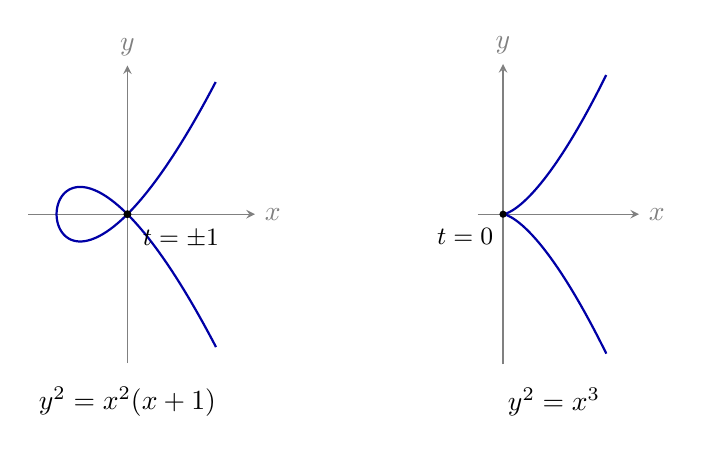
\begin{tikzpicture}[>=stealth,scale=.9]
	\begin{scope}[xshift=0cm]
		\draw[->,gray] (-1.4,0)--(1.8,0) node[right]{\(x\)};
		\draw[->,gray] (0,-2.1)--(0,2.1) node[above]{\(y\)};
		\draw[thick,blue!65!black,domain=-1.5:1.5,samples=151,variable=\t]
			plot ({\t*\t-1},{\t*(\t*\t-1)});
		\fill (0,0) circle (1.6pt);
		\node[below right,font=\small] at (.08,-.08){\(t=\pm1\)};
		\node at (0,-2.65){\(y^2=x^2(x+1)\)};
	\end{scope}
	\begin{scope}[xshift=5.3cm,scale=.8]
		\draw[->,gray] (-.45,0)--(2.4,0) node[right]{\(x\)};
		\draw[->,gray] (0,-2.65)--(0,2.65) node[above]{\(y\)};
		\draw[thick,blue!65!black,domain=-1.35:1.35,samples=121,variable=\t]
			plot ({\t*\t},{\t*\t*\t});
		\fill (0,0) circle (1.8pt);
		\node[below left,font=\small] at (0,-.08){\(t=0\)};
		\node at (.9,-3.31){\(y^2=x^3\)};
	\end{scope}
\end{tikzpicture}

	\caption[结点与尖点的参数模型]{结点与尖点的实点截面。左图参数为 \((t^2-1,t(t^2-1))\)，右图参数为 \((t^2,t^3)\)。}
	\label{g5:fig:node-cusp}
\end{figure}
全局不可约曲线也能在一个点有两个局部分支。为把上面的说法落实到方程，可以允许形式幂级数，即按总次数逐项运算、不讨论数值收敛的级数。在 \(k[[x]]\) 中，方程 \(s(x)^2=1+x\)、\(s(0)=1\) 有唯一解：若 \(s=1+\sum_{r\ge1}c_rx^r\)，逐次比较系数给出
\[
	2c_r=\delta_{r1}-\sum_{i=1}^{r-1}c_i c_{r-i}.
\]
特征不为二保证每步可解。因此在 \(k[[x,y]]\) 中，
\[
	y^2-x^2(x+1)=(y-xs(x))(y+xs(x)).
\]
两个因子分别给出形式图像 \(y=\pm xs(x)\)，每个图像的商环同构于 \(k[[x]]\)，两个因子不是彼此的单位倍。这具体显示了两条形式分支，尽管多项式坐标环本身是整环。

\ProseParagraphBreak

尖点的形式方程则仍不可约。代入 \(x=t^2,y=t^3\) 将
\(k[[x,y]]/(y^2-x^3)\) 嵌入 \(k[[t]]\)：利用 \(y^2=x^3\)，每个类都可唯一写成 \(a(x)+yb(x)\)，其中 \(a,b\in k[[x]]\)。这一归约对幂级数有意义，因为把 \(y^{2r}\) 换成 \(x^{3r}\) 后，对任一固定次数只有有限项贡献。代入后偶次幂与大于等于三的奇次幂不相混，故核为零。商环是整环，因而形式方程有一条分支。这里把形式方程的不可约因子所确定的部分称为形式分支；一般局部环与其完备化的关系将在后续章节系统建立。

\begin{example}\label{g5:exm:nonreduced-point}
	在任意代数闭域 \(k\) 上，方程 \(x=0\) 与 \(x^2=0\) 有同一零点集，商环却分别为
	\[
		k[x]/(x)\simeq k,\qquad
		k[x]/(x^2)\simeq k[\varepsilon]/(\varepsilon^2).
	\]
	后一个环中 \(\varepsilon\ne0\) 而 \(\varepsilon^2=0\)。环中某个正整数次幂为零的元素称为幂零元；没有非零幂零元的环称为约化环。前者是一个约化点的函数环，后者是一个\term[feiyuehuadian]{非约化点}[nonreduced point]的代数模型。作为 \(k\) 向量空间，它们的维数分别为一和二，后一空间的基为 \(1,\varepsilon\)。

	每个到 \(k\) 的 \(k\) 代数同态都把 \(\varepsilon\) 送到零，因而普通 \(k\) 值点看不到这个区别。若允许取值于 \(D=k[\varepsilon]/(\varepsilon^2)\)，则把坐标 \(x\) 送到 \(a\varepsilon\)（\(a\in k\)）都满足 \(x^2=0\)，却只有 \(a=0\) 满足 \(x=0\)。保留这些测试环中的解，就能检测点集中消失的信息。
\end{example}

\subsection{射影闭包中的无穷远分支}
\label{g5:subsec:0105:02}

在 \(\mathbb P_k^2\) 中使用坐标 \([X:Y:Z]\)，把 \(Z\ne0\) 作为原仿射平面。前面两条曲线的射影闭包为
\[
	\overline C_{\mathrm n}=V_+(Y^2Z-X^2(X+Z)),\qquad
	\overline C_{\mathrm c}=V_+(Y^2Z-X^3).
\]
两者在 \(Z=0\) 上都只有 \(P_\infty=[0:1:0]\)。在 \(Y\ne0\) 的图上令 \(u=X/Y,v=Z/Y\)，方程变成
\[
	v-u^3-u^2v=0,\qquad v-u^3=0.
\]
结点模型中 \(1-u^2\) 在 \(P_\infty\) 附近不为零，所以 \(v=u^3/(1-u^2)\)；尖点模型中 \(v=u^3\)。每个模型在无穷远点附近都由一个正则参数 \(u\) 描述，只有一条这样的局部分支。

\ProseParagraphBreak

这也可由射影参数直接核验。将仿射参数写成 \(t=T/S\)，得到
\[
\begin{aligned}
	\nu_{\mathrm n}([S:T])
		&=[S(T^2-S^2):T(T^2-S^2):S^3],\\
	\nu_{\mathrm c}([S:T])
		&=[ST^2:T^3:S^3].
\end{aligned}
\]
两组坐标均为同次齐次多项式，而且在 \(\mathbb P^1\) 上没有公共零点：\(S\ne0\) 时最后一个坐标非零，\(S=0\) 时第二个坐标非零。代入曲线方程检验像确实落在闭包内，且 \(S=0\) 唯一地映到 \(P_\infty\)。这些射影像包含原仿射曲线及其无穷远点，故给出了闭包的全部点。

\begin{example}\label{g5:exm:two-infinity-branches}
	双曲线 \(xy=1\) 的射影闭包为 \(XY=Z^2\)，有两个无穷远点 \([1:0:0]\)、\([0:1:0]\)。在第一点附近用 \(u=Y/X,v=Z/X\)，方程为 \(u=v^2\)；另一点同理。两个点附近各有一条参数分支。参数 \(x=t,y=t^{-1}\) 中的 \(t=0\) 与 \(t=\infty\) 在射影闭包中成为两个不同点。
\end{example}

无穷远点的个数与局部分支的个数须分别判断。把一个结点移到无穷远处即可看到差别：在 \(\overline C_{\mathrm n}\) 中改以直线 \(X=0\) 为无穷远直线，原结点 \([0:0:1]\) 就成为无穷远点，仍带有两条形式分支。由此，齐次化后列出无穷远点只是第一步；还需要在各点的仿射图内查看方程或参数。

\subsection{为什么必须保留局部环和概形纤维}
\label{g5:subsec:0105:03}

一个有理函数能否在指定点延拓，取决于该点附近能否找到不消失的分母。为了把所有这样的函数放在同一对象中，设 \(X\) 为仿射代数集，\(p\in X\)。把包含 \(p\) 的开邻域 \(U\) 上的正则函数 \(f\) 与另一个 \((V,g)\) 视为相同，只要两者在某个更小的 \(p\) 的邻域上相等。所得等价类称为函数在 \(p\) 的\term[hanshuya]{芽}[germ]，其环记为
\[
	\mathcal O_{X,p}=\{\text{在 }p\text{ 附近的正则函数芽}\}.
\]
\symidx{\(\mathcal O_{X,p}\)：\(X\) 在 \(p\) 处的局部环}

\begin{proposition}\label{g5:prop:model-local-ring}
	设 \(k\) 为代数闭域，\(X\) 为仿射代数集，\(p\in X\)，\(A=k[X]\)。每个函数芽都可写成 \(a/b\)，其中 \(a,b\in A\)、\(b(p)\ne0\)。两个这样的分式代表同一芽，当且仅当存在 \(h\in A\)、\(h(p)\ne0\)，使
	\[
		h(ad-bc)=0
	\]
	成立，其中所比较的分式为 \(a/b\) 与 \(c/d\)。此环有唯一极大理想
	\[
		\mathfrak m_p=\{f\in\mathcal O_{X,p}:f(p)=0\},
		\qquad \mathcal O_{X,p}/\mathfrak m_p\simeq k.
	\]
\end{proposition}
\begin{proof}
	分式表达来自正则函数的定义。若两分式在一个邻域内相等，取包含 \(p\) 并位于该邻域内的主开集 \(D(h)\)。函数 \(ad-bc\) 在 \(D(h)\) 上为零，所以 \(h(ad-bc)\) 在整个 \(X\) 上为零。反之，上述等式在 \(D(hbd)\) 上可以除以不消失的分母，给出分式相等。

	求值到 \(k\) 是满同态，其核即 \(\mathfrak m_p\)，因此它是极大理想。若 \(f(p)\ne0\)，在较小邻域上 \(1/f\) 正则，所以 \(f\) 是单位；若 \(f(p)=0\)，求值表明它不可能为单位。因此所有非单位恰组成 \(\mathfrak m_p\)，任何真理想都包含在其中，极大理想唯一。
\end{proof}

只有一个极大理想的交换环称为\term[jubuhuan]{局部环}[local ring]。命题给出的分式环就是记号 \(A_{\mathfrak m}\) 所表示的局部化，其中 \(\mathfrak m=\{a\in A:a(p)=0\}\)。\cref{g5:exm:cusp-local-obstruction}证明了尖点处的局部环不含函数 \(t=y/x\)，而参数直线原点的局部环含有它；局部环由此记录了双有理对应中被遗漏的差别。

\ProseParagraphBreak

一阶测试可以同时检测局部函数及非约化信息。设 \(A=k[x_1,\ldots,x_n]/I\)，并固定一个零点 \(p=(p_1,\ldots,p_n)\)。到双数环 \(D=k[\varepsilon]/(\varepsilon^2)\) 的同态，若模 \(\varepsilon\) 后等于在 \(p\) 的求值，必把坐标送到
\[
	x_i\longmapsto p_i+v_i\varepsilon .
\]
对任意 \(F\in I\)，直接展开每个单项式得到
\[
	F(p+v\varepsilon)=F(p)+
	\varepsilon\sum_{i=1}^n\frac{\partial F}{\partial x_i}(p)v_i.
\]
因而这个赋值能通过商环，当且仅当每个 \(F\in I\) 的一次项都为零。这一解空间是该方程模型在 \(p\) 的\term[Zariskiqiekongjian]{Zariski 切空间}[Zariski tangent space]。计算时只需检查理想生成元：对 \(F=\sum_j a_jF_j\)，因 \(F_j(p)=0\)，一次项就是各 \(F_j\) 一次项的 \(a_j(p)\) 倍之和。

\ProseParagraphBreak

在结点和尖点原点，两方程的一次项都为零，故两者的切空间都是 \(k^2\)；切锥又分别保留了两个方向和一个二重方向。对约化点 \(A=k[x]/(x)\)，一次项条件为 \(v=0\)；对 \(A=k[x]/(x^2)\)，一次项没有约束，得到一维切空间。可见一阶线性化、最低次方程和完整局部环各自保留不同层次的信息。

\begin{example}\label{g5:exm:double-cover-fibres}
	设 \(k\) 为代数闭域且 \(\operatorname{char}k\ne2\)。考虑映射
	\[
		\pi:\mathbb A_k^1\longrightarrow\mathbb A_k^1,\qquad t\longmapsto s=t^2.
	\]
	在 \(s=a\) 上的集合论纤维是方程 \(t^2=a\) 的根集。若直接在坐标环中加入基底方程 \(s-a=0\)，得到纤维代数
	\[
		B_a=k[t]/(t^2-a).
	\]
	当 \(a=b^2\ne0\) 时，\(b\ne-b\)，求值给出同构
	\[
		B_a\longrightarrow k\times k,\qquad f\longmapsto(f(b),f(-b)).
	\]
	其核由 \((t-b)(t+b)\) 生成，满射性可用插值多项式 \((t+b)/(2b)\)、\((b-t)/(2b)\) 核验。当 \(a=0\) 时，
	\(B_0=k[t]/(t^2)\)，有一个二重点。每个 \(B_a\) 都有向量空间基 \(1,t\)，维数恒为二；只取根集，则点数从二变为一。

	特征条件在这里有直接作用：若 \(\operatorname{char}k=2\)，每个 \(a=b^2\) 都满足 \(t^2-a=(t-b)^2\)，所有纤维代数都有非零幂零元。
\end{example}

一般地，若映射由 \(k[s_1,\ldots,s_m]\rightarrow B\)、\(s_i\mapsto f_i\) 给出，在指定点 \(a=(a_1,\ldots,a_m)\) 上保留方程的纤维代数是
\[
	B/(f_1-a_1,\ldots,f_m-a_m).
\]
它满足明确的映射性质：对于任意 \(k\) 代数 \(R\)，从此商环到 \(R\) 的同态，恰对应从 \(B\) 到 \(R\) 且把每个 \(f_i\) 送到 \(a_i\) 的同态。这正是“在基底点上取纤维”对各种测试环应有的含义。把纤维理想替换为其根式再取商，只保留约化的点集结构，会丢掉\cref{g5:exm:double-cover-fibres}中的二重结构。

\ProseParagraphBreak

概形将允许非约化的交换环作为仿射模型，并把这些环的局部信息粘合起来；以上商环随后会成为仿射概形纤维的坐标环。接下来的局部化、有限模与整性理论，分别用于组织点附近的函数、控制代数的有限性，以及比较原曲线和参数曲线。此处各个模型已经显示了这些构造要保留的具体信息。


\begin{chaptersummary}
	多项式环的理想有限生成，使无限方程组可以化成有限方程组，也保证不可约分量只有有限个。零点定理进一步识别点集能够恢复的代数信息：闭集对应根式理想，不可约闭集对应素理想，点对应极大理想。非约化商环中的幂零元需要在点集之外保留。

	\ProseParagraphBreak

	仿射代数集的整体正则函数组成其坐标环，正则映射对应反向的坐标环同态。不可约对象的函数域允许在稠密开集上计算；函数域同构等价于双有理等价，也等价于适当非空开集同构。尖点参数说明，这些条件不能保证整个空间同构，延拓必须检查指定点附近的分母。

	\ProseParagraphBreak

	射影空间由仿射图及正则换图组成，齐次方程保持比例坐标的意义。乘积坐标、全部同次单项式与最大子式分别给出 Segre、Veronese 和 Plücker 嵌入；像的方程与恢复原对象的逆图共同落实了这些构造。射影曲线的参数还允许逐图检查无穷远点。

	\ProseParagraphBreak

	Gröbner 基用首项理想控制除法，Buchberger 判据把检验化为有限对的首项相消。消去理想决定投影像的闭包，饱和去除落在被排除超曲面内的部分；标准单项式则计算有限商代数的维数。局部环记录一个点附近的正则函数，保留方程的纤维代数记录重数及幂零方向，这些计算为后续局部代数和概形构造提供具体对象。
\end{chaptersummary}

\BookExercises

\begin{exercise}\label{g5:ex:radical-embedded-model}
	设 \(k\) 为代数闭域，\(I=(x^2,xy)\subseteq k[x,y]\)。求 \(V(I)\)、\(\sqrt I\)，并说明 \(k[x,y]/I\) 中 \(\overline x\) 非零而幂零。比较在 \(y\ne0\) 的部分与在原点附近，这个元素是否仍可被检测。前一种比较允许 \(y\) 的幂作分母；后一种允许所有 \(h(0,0)\ne0\) 的多项式作分母，元素 \(\overline f\) 变为零指存在这样的 \(h\) 使 \(hf\in I\)。
\end{exercise}
\begin{solution}
	\(x^2=0\) 迫使 \(x=0\)，故 \(V(I)=V(x)\)，零点定理给出 \(\sqrt I=(x)\)。\(\overline x^2=0\)，而 \(x\notin I\)：若 \(x=ax^2+bxy\)，在整环中约去 \(x\) 会得到 \(1=ax+by\)，代入原点矛盾。

	在允许 \(y\) 可逆的商环中，由 \(xy=0\) 得到 \(x=0\)，所以这个幂零元素消失。若在原点局部化后 \(x=0\)，就存在 \(h(0,0)\ne0\) 使 \(hx\in I\)。同样约去 \(x\)，得到 \(h\in(x,y)\)，矛盾。因此它在原点仍非零。这一比较直接使用分式等价关系，显示非约化信息可以集中在一个点附近。
\end{solution}

\begin{exercise}\label{g5:ex:punctured-plane-functions}
	设 \(k\) 为代数闭域，\(U=\mathbb A_k^2\setminus\{(0,0)\}\)。证明每个 \(U\) 上的正则函数都唯一延拓为 \(\mathbb A_k^2\) 上的多项式。进而证明 \(U\) 不同构于任何仿射代数集。
\end{exercise}
\begin{solution}
	\(U=D(x)\cup D(y)\)。由\cref{g5:prop:principal-open-affine}，一个正则函数在两片上分别写成 \(a/x^r\)、\(b/y^s\)，其中 \(a,b\in k[x,y]\)。它们在 \(D(xy)\) 上相同，故整环中有 \(y^sa=x^rb\)。比较关于 \(x\) 的系数，\(x^r\mid a\)，于是函数等于多项式 \(a/x^r\)。稠密性保证延拓唯一。

	若存在同构 \(Z\simeq U\)，其中 \(Z\) 仿射，则复合 \(Z\rightarrow U\hookrightarrow\mathbb A_k^2\) 在整体正则函数环上诱导同构，因为刚证得限制 \(k[x,y]\rightarrow\mathcal O(U)\) 是同构。\cref{g5:thm:affine-morphism-correspondence}遂迫使此复合是到整个 \(\mathbb A_k^2\) 的同构，但它的像遗漏原点，矛盾。
\end{solution}

\begin{exercise}\label{g5:ex:positive-characteristic-bijection}
	设 \(k\) 为特征 \(p>0\) 的代数闭域，考虑 \(F:\mathbb A_k^1\rightarrow\mathbb A_k^1\)、\(t\mapsto t^p\)。证明 \(F\) 在点集上双射，却不是同构，也不是双有理映射。
\end{exercise}
\begin{solution}
	每个 \(a\in k\) 都有 \(p\) 次根；若 \(u^p=v^p\)，则 \((u-v)^p=0\)，域中即有 \(u=v\)。因此 \(F\) 双射。拉回同态 \(k[s]\rightarrow k[t]\) 的像是 \(k[t^p]\)，不含 \(t\)，所以不是环同构，\(F\) 不是同构。

	函数域映射的像为 \(k(t^p)\)。若 \(t=P(t^p)/Q(t^p)\)，其中 \(Q\ne0\)，则 \(tQ(t^p)=P(t^p)\)；左端非零项次数均同余于 \(1\pmod p\)，右端均同余于 \(0\pmod p\)，不可能相等。因此该域嵌入也不满，\(F\) 不是双有理映射。这里结论针对指定映射 \(F\)，其源与靶作为空间当然同构。
\end{solution}

\begin{exercise}\label{g5:ex:dominant-nonsurjective-plane}
	设 \(k\) 为代数闭域，\(\varphi:\mathbb A_k^2\rightarrow\mathbb A_k^2\)、\((x,y)\mapsto(u,v)=(x,xy)\)。求实际像、各点纤维及像的闭包，并写出函数域映射的逆。
\end{exercise}
\begin{solution}
	若 \(u\ne0\)，唯一原像为 \((u,v/u)\)；若 \(u=0,v\ne0\)，没有原像；\((u,v)=(0,0)\) 的纤维则为整条 \(x=0\) 的直线。因此像为 \(D(u)\cup\{(0,0)\}\)，其闭包为整个平面。

	代数上，\(u^iv^j\) 拉回为 \(x^{i+j}y^j\)，不同 \((i,j)\) 得到不同单项式，所以 \(k[u,v]\rightarrow k[x,y]\) 单射。这也确认映射支配。函数域映射有逆 \(x\mapsto u,\ y\mapsto v/u\)，故映射双有理；在 \(x\ne0\) 与 \(u\ne0\) 的开集上实际互逆。支配性及双有理性均不要求所有纤维非空或只有一点。
\end{solution}

\begin{exercise}\label{g5:ex:projective-line-global-functions}
	设 \(k\) 为代数闭域。证明 \(\mathbb P_k^1\) 上每个整体正则函数都是常数，并推得每个正则映射 \(\mathbb P_k^1\rightarrow\mathbb A_k^n\) 都是常值映射。
\end{exercise}
\begin{solution}
	在两张仿射图上分别用 \(t\) 与 \(s=1/t\)。正则函数的限制由\cref{g5:thm:affine-global-functions}分别为 \(f(t)\in k[t]\)、\(g(s)\in k[s]\)。在交上 \(f(t)=g(t^{-1})\)，这在 Laurent 多项式环 \(k[t,t^{-1}]\) 中是恒等式。左端只有非负次数，右端只有非正次数，比较系数可知两者均为相同常数。到仿射空间的正则映射每个坐标函数都常值，结论随即得到。
\end{solution}

\begin{exercise}\label{g5:ex:segre-graph-square}
	设 \(k\) 为代数闭域，\(f:\mathbb P_k^1\rightarrow\mathbb P_k^1\)、\([s:t]\mapsto[s^2:t^2]\)。证明其图像是 \(\mathbb P_k^1\times\mathbb P_k^1\) 中的闭子集，同构于 \(\mathbb P_k^1\)。写出其 Segre 像，并将它与三次 Veronese 曲线比较。
\end{exercise}
\begin{solution}
	在乘积坐标 \(([s:t],[u:v])\) 中，图像由 \(t^2u-s^2v=0\) 给出。如果 \(s\ne0\)，方程强迫 \(u\ne0\) 且 \(v/u=t^2/s^2\)；若 \(s=0\)，则 \(t\ne0,u=0\)，同样唯一确定 \([u:v]\)。所以方程恰好给图像。它在每个仿射乘积图中由多项式方程定义，故闭；第一投影与 \([s:t]\mapsto([s:t],f([s:t]))\) 正则互逆。

	Segre 坐标为
	\[
		[su:sv:tu:tv]=[s^3:st^2:s^2t:t^3].
	\]
	交换中间两个坐标即得 \([s^3:s^2t:st^2:t^3]\)，所以它经射影线性坐标置换成为三次 Veronese 曲线。在特征二时 \(f\) 仍有这些图像与嵌入性质；图像同构由第一投影给出，不要求第二投影 \(f\) 为同构。
\end{solution}

\begin{exercise}\label{g5:ex:grassmann-incidence}
	设 \(k\) 为代数闭域，\(E=\operatorname{span}(e_1,e_2)\subseteq k^4\)。证明 \(\operatorname{Gr}(2,4)\) 中满足 \(W\cap E\ne0\) 的点恰好由 \(p_{34}=0\) 切出。在 \(p_{12}=1\) 的图上，把此条件写成四个矩阵参数的方程。
\end{exercise}
\begin{solution}
	限制到 \(W\) 的投影 \(k^4\rightarrow k^4/E\) 的核是 \(W\cap E\)。选 \(W\) 的一组行基，这个投影的矩阵就是第3、4列；存在非零核恰好等价于该二阶行列式为零，即 \(p_{34}=0\)。

	在指定图上写基矩阵
	\[
		\begin{pmatrix}1&0&a&b\\0&1&c&d\end{pmatrix}.
	\]
	条件为 \(ad-bc=0\)。这是一个四维仿射图中的行列式方程，且与全局 Plücker 超平面方程一致。
\end{solution}

\begin{exercise}\label{g5:ex:division-order}
	在域 \(k\) 上采用字典序 \(x>y\)，用有序列表 \((xy-1,y^2-1)\) 及反向列表分别对 \(xy^2\) 作多元除法。解释为什么余式不同，并求原理想的一个 Gröbner 基。
\end{exercise}
\begin{solution}
	先用 \(xy-1\)，有 \(xy^2-y(xy-1)=y\)，余式为 \(y\)；先用 \(y^2-1\)，有 \(xy^2-x(y^2-1)=x\)，余式为 \(x\)。两余式都不能再由原列表的首单项式整除。差 \(x-y\) 却属于原理想，因为
	\[
		x(y^2-1)-y(xy-1)=y-x.
	\]
	故原列表不是 Gröbner 基。

	理想等于 \((x-y,y^2-1)\)：上式给出一个包含方向，反向由 \(xy-1=y(x-y)+(y^2-1)\) 得到。对这两个首一多项式，
	\[
		S(x-y,y^2-1)=y^2(x-y)-x(y^2-1)=x-y^3
	\]
	先减去 \(x-y\)，再用 \(y^2-1\)，余式为零。因此它们构成 Gröbner 基。
\end{solution}

\begin{exercise}\label{g5:ex:groebner-triple-point}
	设 \(k\) 为代数闭域，\(I=(x^2-y,xy)\subseteq k[x,y]\)，仍取字典序 \(x>y\)。求 Gröbner 基、消去理想 \(I\cap k[y]\)、标准单项式和局部重数，并说明原方程组与消去方程在原点记录的长度为何不同。
\end{exercise}
\begin{solution}
	首项相消给出
	\[
		S(x^2-y,xy)=y(x^2-y)-x(xy)=-y^2.
	\]
	补入 \(y^2\) 后，\(S(xy,y^2)=0\)，而
	\(S(x^2-y,y^2)=-y^3\) 被 \(y^2\) 约为零，故
	\(G=(x^2-y,xy,y^2)\) 是 Gröbner 基。消去定理给出
	\(I\cap k[y]=(y^2)\)，标准单项式为 \(1,x,y\)，商代数长度为三，唯一零点是原点。

	在原商环中 \(y=x^2\)、\(x^3=0\)，所以商环同构于 \(k[x]/(x^3)\)；消去商环 \(k[y]/(y^2)\) 通过 \(y\mapsto x^2\) 嵌入其中，像由 \(1,x^2\) 张成，只有维数二。投影保留了 \(y\) 所能检测的信息，源端还有独立的 \(x\) 方向；两种长度因此不同。
\end{solution}

\begin{exercise}\label{g5:ex:saturation-components}
	设 \(k\) 为代数闭域，\(I=(xy,xz)\subseteq k[x,y,z]\)。证明
	\[
		I=(x)\cap(y,z),\qquad
		I:x^\infty=(y,z),\qquad I:y^\infty=(x).
	\]
	解释各个饱和对应保留了哪一个几何分量。
\end{exercise}
\begin{solution}
	右侧交中的多项式是 \(xf\)，且令 \(y=z=0\) 后为零，于是 \(xf(x,0,0)=0\)，故 \(f(x,0,0)=0\)，即 \(f\in(y,z)\)。反向包含直接成立，因此 \(I\) 为两个素理想的交，其零点集是平面 \(x=0\) 与直线 \(y=z=0\) 的并。

	若 \(x^Nf\in I\)，模 \((y,z)\) 后得到 \(x^N\overline f=0\) 于整环 \(k[x]\)，故 \(f\in(y,z)\)；反向对每个 \(f\in(y,z)\) 都有 \(xf\in I\)。若 \(y^Nf\in I\)，模 \((x)\) 后在 \(k[y,z]\) 中得 \(y^N\overline f=0\)，故 \(f\in(x)\)，反向由 \(xy=0\) 给出。关于 \(x\) 的饱和保留直线，关于 \(y\) 的饱和保留平面，各自去掉完全落在被排除超平面内的那个分量。
\end{solution}

\begin{exercise}\label{g5:ex:closure-intersection}
	设 \(k\) 为代数闭域。在仿射平面取 \(L_0=V(y)\)、\(L_1=V(y-1)\)。求它们在 \(\mathbb P_k^2\) 中的闭包及闭包的交，比较 \(\overline{L_0\cap L_1}\) 与 \(\overline L_0\cap\overline L_1\)。
\end{exercise}
\begin{solution}
	用仿射图 \(Z\ne0\) 的坐标 \(x=X/Z,y=Y/Z\)。两闭包为 \(Y=0\) 与 \(Y-Z=0\) 的射影直线，其交由 \(Y=Z=0\) 给出，是点 \([1:0:0]\)。仿射交为空，因为 \(y=0\) 与 \(y=1\) 不相容，所以 \(\overline{L_0\cap L_1}=\varnothing\)。闭包与有限并相容，却一般不与交相容；本题差别正是新增的无穷远交点。
\end{solution}

\begin{exercise}\label{g5:ex:second-order-directions}
	设 \(k\) 为代数闭域且特征不为二。取 \(R=k[\varepsilon]/(\varepsilon^3)\)，在结点 \(y^2=x^2(x+1)\) 和尖点 \(y^2=x^3\) 的原点分别代入
	\[
		x=a\varepsilon+b\varepsilon^2,\qquad
		y=c\varepsilon+d\varepsilon^2.
	\]
	求满足方程的条件，并解释哪些一阶方向 \((a,c)\) 可提升到这样的二阶解。
\end{exercise}
\begin{solution}
	因为 \(\varepsilon^3=0\)，有 \(x^2=a^2\varepsilon^2\)、\(y^2=c^2\varepsilon^2\)、\(x^3=0\)。结点方程给出 \(c^2=a^2\)，即 \(c=a\) 或 \(c=-a\)；\(b,d\) 任意。尖点方程给出 \(c^2=0\)，域中即为 \(c=0\)，而 \(a,b,d\) 任意。

	在模 \(\varepsilon^2\) 的一阶测试中，两个方程均没有约束，所以切空间同为 \(k^2\)。提升到本题的环后，结点只允许两个切向方向，尖点只允许一个切向方向。这个计算提取了最低次方程，并未声称每个有限阶解都能延拓到全部阶数。
\end{solution}

\begin{exercise}\label{g5:ex:hyperbola-family}
	设 \(k\) 为代数闭域，\(\pi:\mathbb A_k^2\rightarrow\mathbb A_k^1\)、\((x,y)\mapsto xy\)。计算点 \(a\in k\) 上保留方程的纤维代数，分别判断 \(a=0\) 与 \(a\ne0\) 时是否约化、是否不可约、是否连通。
\end{exercise}
\begin{solution}
	纤维代数为 \(B_a=k[x,y]/(xy-a)\)。\(a\ne0\) 时 \(x\) 可逆，\(y=a/x\)，所以
	\[
		B_a\simeq k[x,x^{-1}],
	\]
	它是整环，纤维约化且不可约，因此连通。\(a=0\) 时 \((xy)=(x)\cap(y)\) 为根式理想，纤维仍约化，却由两条坐标轴组成，因而可约。两轴各不可约且在原点相交，所以它们的并连通。本例各纤维都没有非零幂零元，特殊纤维发生的是分量分裂。
\end{solution}

\begin{exercise}\label{g5:ex:direction-map-graph}
	设 \(k\) 为代数闭域，考虑 \(\varphi:\mathbb A_k^2\mathrel{\cdots\!\rightarrow}\mathbb P_k^1\)、\((x,y)\mapsto[x:y]\)。证明它不能在原点正则延拓。证明其图像闭包为
	\[
		B=\{((x,y),[u:v])\in\mathbb A_k^2\times\mathbb P_k^1:xv=yu\},
	\]
	并求第一投影 \(B\rightarrow\mathbb A_k^2\) 在原点的纤维。
\end{exercise}
\begin{solution}
	若有原点邻域上的正则延拓，在 \(x\) 轴的非零部分恒取 \([1:0]\)，由连续性及该点在 \(\mathbb P^1\) 中闭，原点也必须取 \([1:0]\)。沿 \(y\) 轴同理必须取 \([0:1]\)，矛盾。这里原点的任意开邻域在每条轴上都是包含原点的非空开集，除去原点后仍稠密，所用极限结论是 Zariski 闭包意义的。

	图像在 \(B\) 内，且在 \((x,y)\ne(0,0)\) 上比例唯一。对任意 \([u:v]\)，曲线
	\[
		\lambda\longmapsto((\lambda u,\lambda v),[u:v])
	\]
	在 \(\lambda\ne0\) 时位于图像，在 \(\lambda=0\) 时给出 \(((0,0),[u:v])\)。非零参数在仿射直线上稠密，所以这一点也在图像闭包内，证明闭包就是 \(B\)。因此原点纤维为整个 \(\mathbb P^1\)。在 \(u\ne0\) 的图上令 \(w=v/u\)，方程为 \(y=xw\)；在 \(v\ne0\) 的图上同理为 \(x=y(u/v)\)，可以直接查看新增的方向参数。
\end{solution}

\begin{exercise}\label{g5:ex:quotient-multiplication}
	设 \(k\) 为代数闭域，\(I=(x^2-y,y^2)\subseteq k[x,y]\)。分别在字典序 \(x>y\) 和 \(y>x\) 下求 Gröbner 基及标准单项式；在有序基 \((1,x,y,xy)\) 上写出商代数中乘以 \(x\)、乘以 \(y\) 的矩阵。比较这个商代数与 \(k[x,y]/(x^2,y^2)\)：它们是否有相同长度，是否同构？
\end{exercise}
\begin{solution}
	在 \(x>y\) 时，\(G=(x^2-y,y^2)\) 的唯一一对 \(S\) 多项式为 \(-y^3\)，可约为零，标准单项式是 \(1,x,y,xy\)。在 \(y>x\) 时，可改写理想为 \((y-x^2,x^4)\)；其 \(S\) 多项式为 \(-x^6\)，同样可约为零，标准单项式为 \(1,x,x^2,x^3\)。

	以矩阵的第 \(j\) 列记录第 \(j\) 个基向量的像，乘法矩阵为
	\[
		M_x=\begin{pmatrix}
			0&0&0&0\\1&0&0&0\\0&1&0&0\\0&0&1&0
		\end{pmatrix},\qquad
		M_y=M_x^2=\begin{pmatrix}
			0&0&0&0\\0&0&0&0\\1&0&0&0\\0&1&0&0
		\end{pmatrix}.
	\]
	原商代数同构于 \(k[x]/(x^4)\)，唯一极大理想 \(\mathfrak m\) 满足 \(\mathfrak m^3\ne0,\mathfrak m^4=0\)。另一商代数也有基 \(1,x,y,xy\)，故两者长度均为四；但其唯一极大理想 \(\mathfrak n=(\overline x,\overline y)\) 满足 \(\mathfrak n^2=k\overline{xy}\ne0,\mathfrak n^3=0\)。环同构必须保持唯一极大理想及其各次幂，故二者不同构。长度相同并不确定乘法。
\end{solution}
